\documentclass[11pt]{aghdpl}
% \documentclass[language=en,11pt]{aghdpl}  % praca w języku angielskim


%---------------------------------------------------------------------------

\author{Piotr Seemann}
\shortauthor{P. Seemann}

%\titlePL{Przygotowanie bardzo długiej i pasjonującej pracy dyplomowej w~systemie~\LaTeX}
%\titleEN{Preparation of a very long and fascinating bachelor or master thesis in \LaTeX}

\titlePL{Automatyczne odkrywanie procesów biznesowych przy użyciu programowania genetycznego}
\titleEN{Automated Business Process Discovery using Genetic Programming}


\shorttitlePL{Automatyczne odkrywanie procesów biznesowych przy użyciu programowania genetycznego} % skrócona wersja tytułu jeśli jest bardzo długi
\shorttitleEN{Automated Business Process Discovery using Genetic Programming}

\thesistype{Projekt dyplomowy}
%\thesistype{Master of Science Thesis}

\supervisor{dr inż. Krzysztof Kluza}

\degreeprogramme{Informatyka}
%\degreeprogramme{Computer Science}

\date{2021}

\department{Katedra Informatyki Stosowanej}
%\department{Department of Applied Computer Science}

\faculty{Wydział Elektrotechniki, Automatyki,\protect\\[-1mm] Informatyki i Inżynierii Biomedycznej}
%\faculty{Faculty of Electrical Engineering, Automatics, Computer Science and Biomedical Engineering}

\setlength{\cftsecnumwidth}{10mm}

%---------------------------------------------------------------------------
\setcounter{secnumdepth}{4}
\brokenpenalty=10000\relax

\begin{document}

\titlepages

\RedefinePlainStyle

\setcounter{tocdepth}{2}
\tableofcontents
\clearpage


\chapter{Wprowadzenie}
\label{cha:wprowadzenie}

%---------------------------------------------------------------------------

\section{Zarys tematyki pracy}
\label{sec:zarysPracy}

Zdefiniowanie kroków potrzebnych do osiągnięcia danego efektu jest konieczne do zrozumienia podejmowanych działań i wprowadzenia ewentualnych udoskonaleń. Z czasem biznes zdał sobie z tego sprawę i kierując się zasadą: ,,Jeżeli nie jesteś w stanie opisać czegoś jako proces, nie masz pojęcia, co robisz'', firmy zaczęły podejmować próby uporządkowania i zamknięcia swoich działań w ramy, co doprowadziło do wzrostu popularności procesów biznesowych.

Identyfikacja i opis procesów biznesowy sprawia, że wszystkie operacje w firmie stają się przejrzyste i łatwiejsze do zrozumienia. Analiza procesów biznesowych może pozwolić na zwiększenie produktywności oraz redukcję kosztów. Procesy biznesowe mogą pozwolić na przewidywanie przyszłych zdarzeń na podstawie danych, znajdowanie wąskich gardeł, a także zmniejszają zależność firm od poszczególnych ludzi.

W związku z możliwością gromadzenia coraz większej ilości danych, a także chęcią ich wykorzystania oraz rosnącą popularnością analizy danych (\textit{eng. data science}), biznes zdał sobie sprawę z możliwości wykorzystanie technologii informatycznych w kontekście procesów biznesowych. Zapoczątkowało to powstanie na pograniczu zarządzania procesami biznesowymi i metod informatycznych używanych do analizy danych, wśród wielu innych, dziedziny zwanej eksploracją procesów (\textit{eng. process mining}).
 
\section{Cele pracy}
\label{sec:celePracy}

Celem pracy jest projekt i implementacja metody odkrywania procesów biznesowych przy użyciu programowania genetycznego, a dokładniej ewolucji gramatycznej. W ramach pracy zaimplementowano program realizujący to zadanie oraz zbadano jak wybór metryk, metod ewolucji, gramatyki, a także parametrów programu wpływa na jakość rozwiązania. Działanie zweryfikowano poprzez użycie stworzonego algorytm do okrycia modeli procesów biznesowych dla dzienników zdarzeń różnej wielkości. Przykłady czego zamieszczono i omówiono w pracy. Ponadto w pracy została zbadana hipoteza, czy kontrola złożoności modelu na etapie ewolucji ma korzystny wpływ na działanie algorytmu i ostateczne rozwiązanie.
%---------------------------------------------------------------------------

\section{Zawartość pracy}
\label{sec:zawartoscPracy}

Praca zastała podzielona na cztery części. We wstępie teoretycznym zostały przybliżone zagadnienia potrzebne do zrozumienia pracy, takie jak procesy biznesowe, eksploracja procesów oraz ewolucja gramatyczna. Omówiono też wybór i działanie metryk dla modeli procesów biznesowych. W kolejnej części została przedstawiona gramatyka stworzona na potrzebny odkrywania procesów oraz projekt i implementacja algorytmu do wyszukiwania procesów genetycznych. Następnie zaprezentowane zostały wyniki działanie algorytmu dla przykładowych dzienników zdarzeń. Sprawdzone zostało jak na czas znajdowania rozwiązania oraz jego jakość wpływają przyjęte parametry algorytmu w szczególności wybór metryk, oraz wagi, z jakimi każda metryka powinna być brana pod uwagę. Zweryfikowana została hipoteza dotycząca złożoności modelu. Na koniec przedstawiono podsumowanie całości pracy. 



















\chapter{Wstęp teoretyczny}
\label{cha:wstepTeoretyczny}

W celu wprowadzenia do tematyki odkrywania procesów biznesowych oraz programowania genetycznego w tej części zostały przybliżone niezbędne zagadnienia teoretyczne. Zaprezentowana tematyka obejmuje procesy biznesowe, zarządzanie nimi oraz ich eksplorację. Przedstawiono również notacje używaną  do reprezentowania procesów w~dalszej części pracy. Następnie, przybliżono programowanie genetyczne oraz ewolucję gramatyczną, a także omówiono, jakiej gramatyki używać w tej technice. Do oceny jakości modelu konieczne są metryki, dlatego opisano używane metryki i pokazano, jak je obliczać.


%---------------------------------------------------------------------------

\section{Procesy biznesowe}
\label{sec:procesyBiznesowe}

W każdym dużym przedsiębiorstwie codziennie wykonywana jest ogromna ilość czynności koniecznych do funkcjonowania tej organizacji. Ludzie oraz systemy realizują rozmaite działania związane~z~różnymi, często niemającymi wiele wspólnego zadaniami, jak np. przetwarzanie płatności, składnie zamówień, wytwarzanie produktów czy ich transport. Przykłady te można mnożyć w zależności od~sektora, do~jakiego należy dana firma. Im jest ona większa, tym trudniej jest osobom nią zarządzającym zrozumieć i opisać poszczególne czynności. W pewnym momencie, kiedy ilość różnych zadań rośnie do~setek czy tysięcy, staje się to niemożliwe i potrzebny jest sposób na zebranie wiedzy o pojedynczych operacjach i zamknięcie ich w uporządkowaną strukturę. Stąd narodził się pomysł na wykorzystanie procesów biznesowych.

Procesy biznesowe opisują zbiór aktywności, które podejmuje grupa podmiotów w celu osiągnięcia celu biznesowego. W literaturze brakuje jednej ogólnie przyjętej definicji procesu biznesowego. W latach 90. XX wieku orędownicy BPR, czyli przeprojektowania procesów biznesowych (\textit{ang. Business Process Re-engineering}) starali się sprecyzować pojęcie procesu biznesowego. W książce ,,Process Innovation: Reengineering Work through Information Technology''~\cite{davenport1993process} określono termin ten jako: \textit{,,Ustrukturyzowany, mierzalny zbiór działań, których celem jest wytworzenie określonego produktu dla określonego klienta lub rynku''}. Autor położył nacisk na zbiór kroków prowadzących do celu, raczej niż na końcowy efekt. W dalszej części podsumowano: \textit{,,Proces jest zatem określonym uporządkowaniem czynności roboczych w czasie i przestrzeni, z początkiem i końcem oraz jasno określonymi wejściami i wyjściami: strukturą działania.''}. Inni pionierzy BPR Michael Hammer i James Champy zdefiniowali proces biznesowy jako: \textit{,,zbiór działań, który pobiera jeden lub więcej rodzajów danych wejściowych i tworzy wynik, który ma wartość dla klienta''}~\cite{HAMMER199390}. Autorzy dają większą dowolność, co do definicji procesu, nie wspominając o konieczności jego logicznej organizacji czy mierzalności. Z kolei Ivar Jacobson zupełnie pomija konieczność zamknięcia procesu w jakiekolwiek ramy, określając go jako: \textit{,,Zestaw czynności wewnętrznych wykonywanych w celu obsługi klienta''}~\cite{JacobsonObjectAdvantage}. Nacisk na konieczność odniesienia procesów do wymiernych środków firmy widzimy w definicji zaproponowanej przez Hans-Erika Erikssona: \textit{,,Procesy biznesowe są aktywną częścią biznesu. Opisują funkcje firmy i obejmują zasoby, które są używane, przekształcane lub wytwarzane. Proces biznesowy to abstrakcja, która pokazuje współpracę między zasobami~i~transformację zasobów w biznesie. Podkreśla, w jaki sposób wykonywana jest praca, zamiast opisywać produkty lub usługi wynikające z tego procesu.''}~\cite{Eriksson2000BusinessMW}. Szczególnie ważny jest tutaj fragment~o~transformacji zasobów, gdyż każe on rozumieć poszczególne aktywności w procesie jako powiązane ze sobą~i~kończące się namacalnymi rezultatami. Definicja \textit{,,Proces biznesowy to seria kroków mających na celu wytworzenie produktu lub usługi. W wyniku niektórych procesów produkt lub usługa jest odbierana przez zewnętrznego klienta organizacji. Nazywamy je podstawowymi procesami. Inne procesy wytwarzają produkty, które są niewidoczne dla klienta zewnętrznego, ale są niezbędne do efektywnego zarządzania firmą. Nazywamy je procesami wsparcia''}~\cite{rummler_brache_1995} wprowadza rozgraniczenie na podtypy procesów. Ważnym jest jednak, że nie jest koniecznością, aby rezultaty procesu były widoczne na zewnątrz organizacji. Warto też zaznaczyć, że procesy biznesowe nie dotyczą jednej osoby czy nawet działu,~a~raczej udział w nich bierze wiele ludzi, maszyn czy systemów z różnych działów połączonych celem dostarczenia wspólnej wartości biznesowej.

Powyższe definicje skupiają się na odmiennych aspektach procesów biznesowych, nie zawsze szczegółowo wspominając o innych. Starając się usystematyzować powyższe sformułowania, chcąc zbudować bazę do dalszej analizy tematu, można przyjąć, że procesy biznesowe charakteryzują:
\begin{itemize}
  \item[•] Określony cel, którym jest wytworzenie wartości dla klienta zewnętrznego lub pośrednio firmy -- klienta wewnętrznego. Jednak warto jeszcze raz zaznaczyć, że proces biznesowy skupia się na~sposobie osiągnięcia celu, a nie opisie celu samego w sobie. 
  \item[•] Dyskretny, jasno zdefiniowany i identyfikowalny zbiór aktywności. 
  \item[•] Jasno określony początek -- wejście i koniec -- wyjście.
  \item[•] Zależność przyczynowo-skutkowa pomiędzy kolejnymi aktywnościami.
\end{itemize}

Aby lepiej zilustrować, czym jest proces biznesowy, na rys. \ref{fig:simple_business_process} znajduje się prosty przykład często spotykanego procesu.

\begin{figure}[H]
	\centering{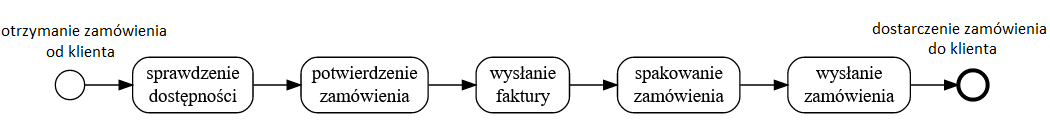
\includegraphics[scale=0.57]{simple-process-new.png}}
	\caption{\label{fig:simple_business_process}Przykład prostego procesu}
\end{figure}

Zauważmy, że mamy jasno zdefiniowany wejście -- otrzymanie zamówienia od klienta oraz wyjście, kiedy dostarczamy oczekiwaną wartość dla klienta, a całość składa się z serii tworzących logiczną całość aktywności. Są one konkretnie zdefiniowane.

Zdefiniowanie procesu biznesowego otwiera wiele możliwości analizy działań przedsiębiorstwa~i~wskutek tego wprowadzanie usprawnień. Dziedziną, która się tym zajmuje, jest zarządzanie procesami biznesowymi (\textit{ang. Business Process Managment}) zwane w skrócie BPM. Sercem jest proces,~a~samo BPM jest dyscypliną używającą różnych metod, technik i sposobów w celu projektowania, wprowadzania w życie, zarządzania i analizy procesów biznesowych~\cite{BPMDemystified}. 

Celem stosowania metod zarządzania procesami biznesowym jest udoskonalanie procesów w danej organizacji biznesowej. Udoskonalanie może być rozumiane w różnoraki sposób w zależności od~kierunku rozwoju firmy. Może to być na przykład redukcja czasu, kosztów, czy dostarczanie lepszego produktu końcowego. Ważne jest, aby było to podejście całościowe i odnosiło się do całego zbioru aktywności w ramach danego procesu. Usprawnianie pojedynczej aktywności to nie jest BPM. Patrząc na~przykład powyżej, jeśli wprowadzono by usprawnienia w ramach wysyłania faktury, robiąc to elektronicznie zamiast tradycyjną pocztą, mimo że taka zmiana przyniosłaby poprawę wydajności, nie byłoby to zarządzaniem procesami biznesowymi. O BPM można by mówić, gdyby znaleziono sposób, żeby przeprojektować cały proces tak, aby wysyłanie faktury nie było potrzebne lub odwrotnie, jeśli dodano by nowe aktywności, co usprawniłoby proces jako całość czy nawet zmieniono kolejności zdarzeń w procesie, gdyż zmiana ilości poszczególnych, jednostkowych aktywności nie są konieczna, żeby ulepszyć proces jako całość \cite{BPMWhat}.

Zarządzanie procesami biznesowymi jest zbiorem praktyk mających na celu udoskonalanie procesów. Trzeba więc rozumieć BPM jako pojęcie abstrakcyjne, jednak szczególnie w dzisiejszym świecie, zarządzanie procesami biznesowymi nie może się obyć bez wsparcia ze strony oprogramowania czy technik znanych z różnych dziedzin informatyki \cite{BPMSurvey}.

\begin{figure}[H]
	\centering{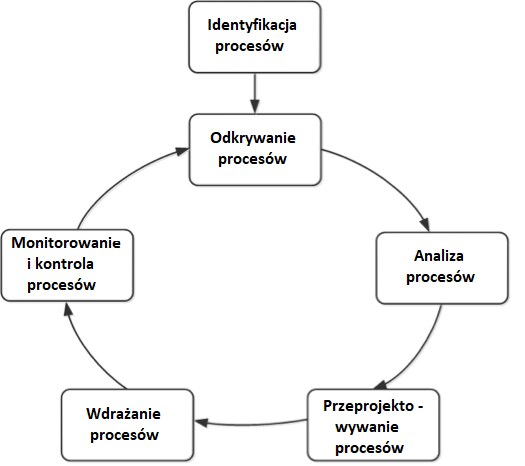
\includegraphics[scale=0.55]{lifecycle.png}}
	\caption{\label{fig:lifecycle}Cykl życia procesu biznesowego \cite{dumas2013fundamentals}}
\end{figure}

Cykl życia procesu biznesowego (\textit{ang. Business Process Lifecycle}) przedstawiono na rys. \ref{fig:lifecycle}. Jest to~zbiór kroków niezbędnych do skutecznego zarządzania procesami biznesowymi. W celu dostosowania do zmieniającej się rzeczywistości poszczególne kroki powinny być co pewien czas powtarzane. Konieczność powtarzania elementów cyklu życia procesu biznesowego sygnalizuje przewagę komputerów~i~algorytmów nad wykonywaniem tych operacji przez człowieka. Metody informatyczne są~stosowane na każdym z wymienionych etapów. W szczególności dane zebrane w wyniku monitorowania procesów dają możliwość zastosowania metod z zakresu eksploracji procesów (sekcja \ref{sec:eksploracja}). Praca skupia się w~głównej mierze na odkrywaniu procesów, czyli znajdowaniu istniejących już procesów na podstawie realnych danych. Należy zaznaczyć, że identyfikacja polega na ogólnym rozpoznaniu~i~nazwaniu zachodzących procesów, podczas gdy odkrywanie jest bardziej szczegółowe, a w jego wyniku otrzymujemy dokładny model.  

%---------------------------------------------------------------------------

\section{Metody modelowania i eksploracji procesów}
\label{sec:eksploracja}
W tej sekcji rozwinięto tematykę procesów biznesowych o~metody ich modelowania oraz eksploracji na podstawie danych zawartych w dziennikach zdarzeń.

\subsection{Modelowanie procesów biznesowych}
\label{sec:modelling}
Na rys. \ref{fig:simple_business_process} przedstawiono przykład uproszczonego procesu biznesowego. Łatwo sobie wyobrazić, że proces ten w rzeczywistości może być znacznie bardziej skomplikowany. Część aktywności może być wykonywana równolegle, niektóre zdarzenia w ogóle nie zaistnieją lub będą występować kilkukrotnie~w~ramach jednego procesu. 

W sytuacji, w której zamówiony przez klienta towar będzie niedostępny, logiczne wydaje się poinformowanie go o opóźnieniu oraz danie mu możliwości anulowanie zamówienia lub jego kontynuacja~i~ponowne sprawdzenie dostępności. Ponadto, czynności takie jak wysłanie faktury oraz spakowanie~i~wysłanie zamówienia mogą być wykonane w dowolnej kolejności czy nawet jednocześnie przez dwie różne osoby. Proces staje się bardziej skomplikowany i konieczna do stworzenia jego modelu jest bardziej złożona notacja niż użyta do przedstawienia najprostszego procesu. 
Istnieje wiele notacji do modelowania procesów biznesowych, wśród nich można wymienić schematy blokowe, diagramy aktywności UML, łańcuchy procesu sterowanego zdarzeniami (\textit{eng. Event-driven Process Chains}), sieci Petriego \cite{BPMComparission}. Obecnie najpopularniejszą notacją używaną do opisu procesów biznesowych jest Business Process  Model and Notation, w skrócie BPMN \cite{omg2011bpmn}. Daje ona możliwość opisania w jednoznaczny sposób skomplikowanych procesów czy stworzenia diagramów współdziałania procesów, jednocześnie pozostając łatwą do zrozumienia.

Na grafice na rys. \ref{fig:bpmn_example} przedstawiono notację opartą o elementy BPMN, używaną w dalszej części pracy. Składają się na nią zdarzenia początkowe i końcowe, połączenia, bramki logiczne oraz aktywności. Bramki LUB oraz ALBO mogą zostać pominięte, co pokazano dla bramki LUB. Podobnie pętle mogą zostać wykonane zero razy.

\begin{figure}[H]
	\centering{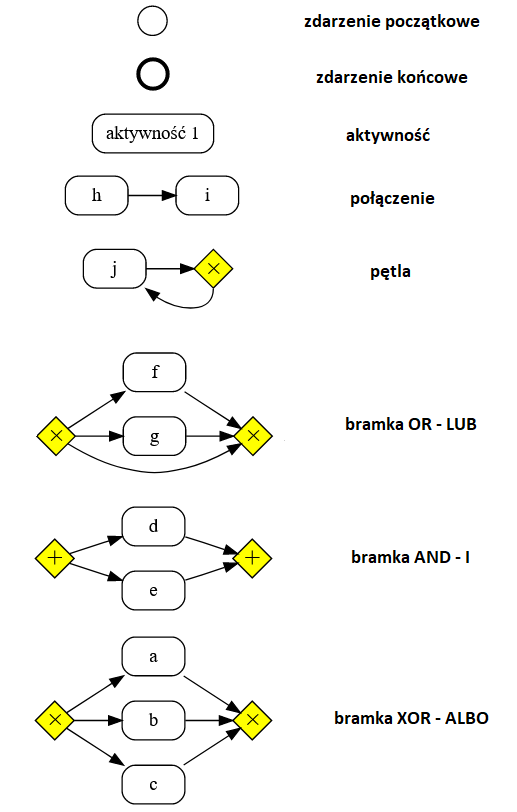
\includegraphics[scale=0.4]{BPMNelements.png}}
	\caption{\label{fig:bpmn_example}Elementy składające się na notację}
	\label{fig:lifecycle}
\end{figure}

Korzystając z tej notacji, można przedstawić opisany wcześniej proces. Na rys.  \ref{fig:complicated_business_process_1} widać model po~modyfikacjach. 

\begin{figure}[h]
	\centering{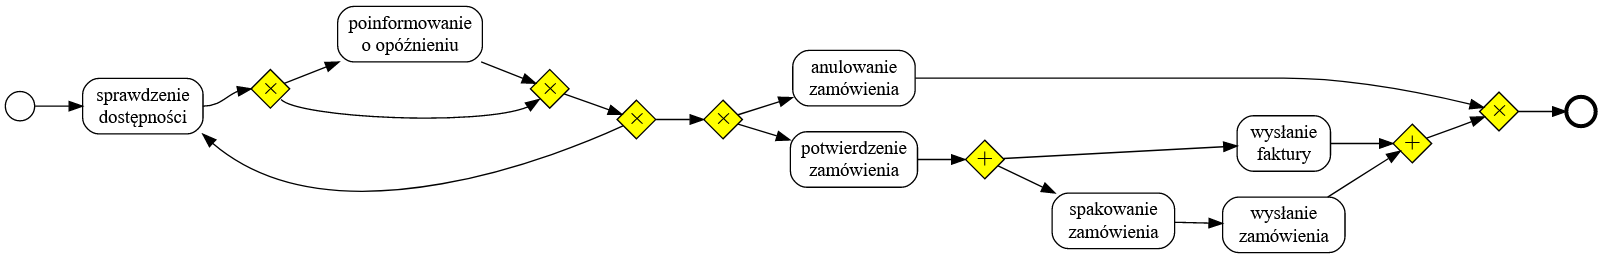
\includegraphics[scale=0.28]{complicated-process-example-1-new2.png}}
	\caption{\label{fig:complicated_business_process_1}Rozbudowany model procesu -- przykład 1}
\end{figure}

Możliwe jest teraz poinformowanie klienta o opóźnieniu, a następnie anulowanie zamówienia lub powtórne sprawdzenie dostępności. Model ten jednak nie jest wystarczająco precyzyjny i pozwala na~potwierdzenie zamówienia po informacji o jego opóźnieniu, a bez uprzedniego ponownego sprawdzenia dostępności. Można zaproponować inny model (rys. \ref{fig:complicated_business_process_2}), który rozwiązuje powyższe problemy, jednak aktywność -- poinformowanie o opóźnieniu -- występuje w nim dwukrotnie, co jest niepożądane i pogarsza jego czytelność.

\begin{figure}[h]
	\centering{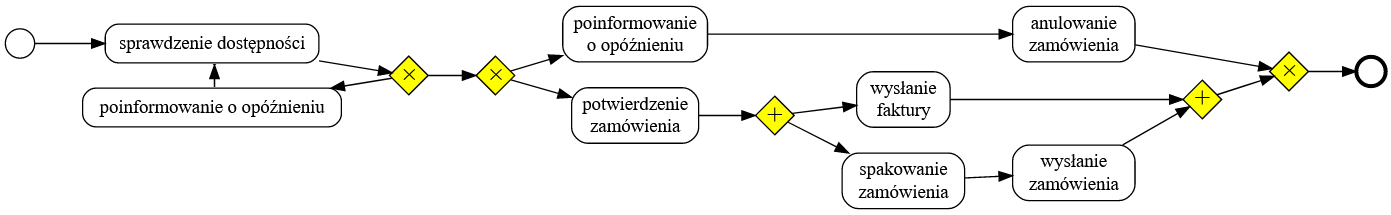
\includegraphics[scale=0.39]{complicated-process-example-2-new2.png}}
	\caption{\label{fig:complicated_business_process_2}Rozbudowany model procesu -- przykład 2}
\end{figure}

Niewykluczona jest również sytuacja, że w pewnych przypadkach możliwe jest anulowanie zamówienia bez uprzedniego poinformowania klienta o opóźnieniu, a~z~czego nie zdawano sobie sprawy na~etapie tworzenia modelu. Wtedy konieczne będzie przemodelowanie procesu. Aby radzić sobie z~tymi problemami i~tworzyć lepsze modele, powstał szereg zestawów wytycznych, którymi warto się kierować, modelując procesy biznesowe. Wśród takich zasad można wymienić: zminimalizuj liczbę elementów w~modelu, zminimalizuj liczbę ścieżek w~modelu, używaj jednego zdarzenia początkowego i jednego końcowego, unikaj bramek LUB, zdekomponuj model zawierający więcej niż 50 elementów \cite{7PMG}.

Modelowania procesów biznesowych jest próbą stworzenia uproszonej wersji rzeczywistości na podstawie przewidywań i założeń. Modele dają użyteczne przybliżenie rzeczywistości, jednak należy pamiętać, że \textit{,,wszystkie modele są błędne''} i rzeczywisty proces najprawdopodobniej będzie różnił się od~nawet najlepszego modelu. 


\subsection{Eksploracja procesów}

W dzisiejszych czasach standardem jest, że organizacje biznesowe korzystają z systemów informatycznych, takich jak systemy ERP czy CRM, wspierających ich działalność. Systemy te rejestrują dane~o~procesach, które wspierają. Dane te mogą być później analizowane i wykorzystane do wprowadzenia usprawnień w działaniu firmy.   

Tradycyjne, ręczne modelowanie procesów jest wolne, kosztowne i narażone na błędy ludzkie, a~konieczność ciągłego powtarzania tej czynności, połączona z wszechobecnym w~biznesie trendem automatyzacji sprawiają, że eksploracja procesów zyskuje na znaczeniu \cite{market-pm}. Ważna jest możliwość szybkiej adaptacji do~zmian, a~automatyzacja odkrywania procesów biznesowych pozwala na wykonywanie powtarzalnych zadań, eliminując przy tym błędy, co idealnie wpisuje się w ten trend.

Eksploracja procesów jest to szeroko pojęta dziedzina, która zawiera różne aplikacje inteligencji obliczeniowej, uczenia maszynowego i eksploracji danych do modelowania i analizy procesów. 
Jest wartościowym dodatkiem do innych metod eksploracji danych, gdyż zamiast skupiać się pojedynczym rezultacie i tworzyć dotyczące jego predykcje, celem jest poznanie akcji, które prowadzą do końcowego wyniku. Jest to trudniejsze, ale wyjątkowo cenne z punktu widzenia biznesowego, gdyż jakakolwiek zmiana w trakcie procesu może sprawić, że przewidywania będą kompletnie nietrafione, a  zrozumienie całego procesu pozwala na pełniejszy obraz i łatwiejsze dostosowywanie się do zmian. 

Procesy biznesowe są zazwyczaj domeną analityków i menadżerów, którzy nie zawsze podchodzą do tematu ich analizy w sposób ścisły i mający odniesie w faktach, często opierając się na własnych przeczuciach czy doświadczeniach, wprowadzając czynnik ludzki, który może być przyczyną błędów. Stworzenie pomostu między metodami informatycznymi a~biznesem i~stworzenie możliwości na ścisłe, powtarzalne~i~sprawdzalne analizowanie procesów jest więc nad wyraz cenne. Eksploracja procesów biznesowych oparta jest bowiem na danych i~nie ma w~niej wiele miejsca na przypuszczenia~i~domysły.

Na eksplorację procesów składają się techniki, narzędzia oraz metody odkrywania, monitorowania~i~usprawniania rzeczywistych procesów poprzez wiedzę wyodrębnioną z~dzienników zdarzeń powszechnie dostępnych w~systemach informatycznych \cite{pm-manifesto, mining-overview}.
Wyróżnia się trzy podkategorie: 
\begin{itemize}
  \item[•] automatyczne odkrywanie procesów (\textit{ang. process discovery}),
  \item[•] sprawdzanie zgodności (\textit{ang. conformance checking}),
  \item[•] udoskonalanie procesu (\textit{ang. performance mining}).
\end{itemize}


\subsection{Dzienniki zdarzeń}
\label{sec:event_logs}
Danymi wejściowymi dla algorytmów z dziedziny eksploracji procesów są dzienniki zdarzeń, zwane często logami. Przykład przedstawiono na rys. \ref{fig:event_log_example}.
 
\begin{figure}[h]
	\centering{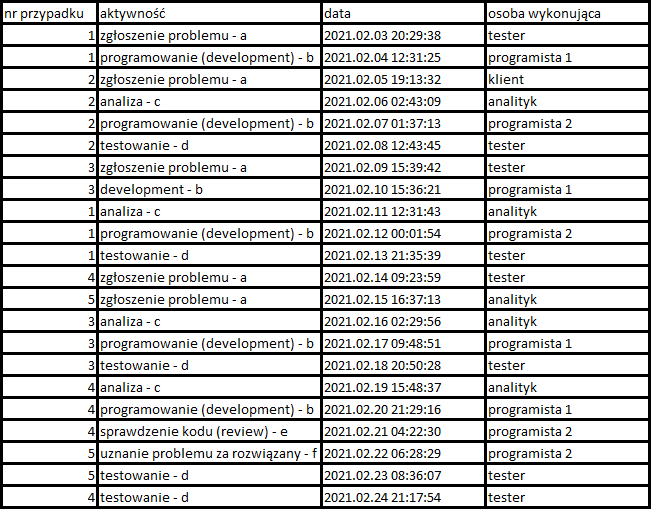
\includegraphics[scale=0.6]{event-log-example-2.png}}
	\caption{\label{fig:event_log_example}Przykład dziennika zdarzeń}
\end{figure}

Przyjmuje się, że aby mówić o dzienniku zdarzeń powinien on zawierać trzy informacje niezbędne w kontekście odkrywania procesów biznesowych: numer przypadku, czyli unikalny identyfikator zbioru aktywności, nazwę aktywności oraz datę jej wykonania -- ważną tylko w kontekście kolejności wykonywania pojedynczych aktywności. Ponadto może on zawiera inne dodatkowe informacje, takie jak: podmiot wykonujący daną aktywność, miejsce, koszt czy aktualny postęp wykonania. Te~pozostałe dane mogą być wykorzystywane w kolejnych etapach analizy i usprawniania procesu.

Mając do dyspozycji te trzy informacje -- poszczególne przypadki, aktywności na~nie się składające oraz ich kolejność, zliczane jest, jak często poszczególne aktywności występują w danej kolejności. Każdy taki uporządkowany zbiór aktywności zwany jest wariantem procesu. Przykład odpowiadający dzienniki zdarzeń pokazanemu w tej sekcji przedstawiono na rys. \ref{fig:process_variants_example}.

\begin{figure}[H]
	\centering{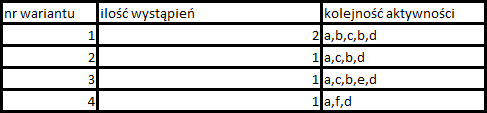
\includegraphics[scale=0.6]{variants-example.png}}
	\caption{\label{fig:process_variants_example}Warianty procesu odpowiadające przykładowemu dziennikowi zdarzeń}
\end{figure}

Dla poprawy czytelności aktywności często reprezentowane są jako symbole, np. kolejne litery alfabetu, zamiast pełnej nazwy.

\subsection{Automatyczne odkrywanie procesów biznesowych}
\label{sec:discovery}

Automatyczne odkrywanie procesów biznesowych jest poddziedziną eksploracji procesów i~obejmuje techniki przekształcania danych w procesy. Wejściem jest dziennik zdarzeń, a wyjściem mapa lub model procesu. Ważne jest, żeby proces był oparty na analizie prawdziwych danych, a nie spekulacjach i~założeniach. Automatyczne odkrywanie procesów pozwala na znajdowanie procesu takim, jaki jest, a~nie takim, jakim chciano by, żeby był.

Celem automatycznego odkrywania procesów biznesowych jest zaprojektowanie funkcji -- algorytmu, która przekształci dane z dziennika zdarzeń w model procesu \cite{pm-book}. Istnieje wiele algorytmów do odkrywania procesów biznesowych. Wśród najpopularniejszych można wymienić:
\begin{itemize}
  \item[•] Alpha algorithm \cite{alpha-algorithm},
  \item[•] The ILP Miner \cite{ILP-miner},
  \item[•] Heuristic Miner \cite{heuristics-miner},
  \item[•] Multi-phase Miner \cite{multi-phase-miner},
  \item[•] Inductive Miner \cite{inductive-miner}.
\end{itemize}

Istnieją cztery powszechnie używane kryteria do określania jakości otrzymanego modelu. Konieczne jest znalezienie balansu między nimi, gdyż często starając się poprawiać model pod kątem jednego kryterium, pogorszy się on pod względem innych. Powstało wiele metryk przedstawiających je za pomocą wzorów matematycznych \cite{conf-propositions, Blum2015MetricsIP}. Bardziej szczegółowo wybór metryk omówiono w sekcji \ref{sec:metryki}, a~poniżej przedstawiono jedynie krótki opis poszczególnych kryteriów:
\begin{itemize}
  \item[•] odwzorowanie (\textit{ang. fitness}) -- zgodność modelu z dziennikiem zdarzeń,
  \item[•] prostota (\textit{ang. simplicity}) -- złożoność i łatwość zrozumienia modelu,
  \item[•] precyzja (\textit{ang. precision}) -- brak zachowań niezwiązanych z logiem, a możliwych w modelu,
  \item[•] generalizacja (\textit{ang. genralization}) -- odzwierciedlenie w modelu brakujących aktywności z powodu niekompletnego logu.
\end{itemize}


Wśród problemów dotykających istniejące algorytmy można wymienić problem ze znajdowaniem aktywności zachodzących równolegle, brak możliwości pomijania aktywności czy reprezentowania duplikatów, nieradzenie sobie z zakłóceniami w logu, tworzenie zbyt skomplikowanych modeli, czy trudność z odwzorowaniem niektórych zachowań. Modele stworzone mogą nie być spójne strukturalnie~\mbox{\cite{dongen2006b, StructuralDetectionofDeadlocks}}, przez co rozumie się modele, w których istnieje aktywność, z której nie możemy osiągnąć zdarzenia końcowego lub nie może być ona w żaden sposób osiągnięta ze zdarzenia początkowego. Metody te zazwyczaj oparte są na grafach bezpośrednich następstw (\textit{ang. directly follows graphs}), przez co problemem może być sytuacja, kiedy log jest niekompletny. 

Zastosowanie algorytmów genetycznych do automatycznego odkrywania procesów biznesowych może być odpowiedzią na te kłopoty. Takie podejście pozwala na wyeliminowanie części problemów często dotyczących innych metod. Najważniejszą jednak przewagą algorytmów genetycznych jest pełna dowolność w kwestii generowania modelu pod kątem metryk zdefiniowanych przez użytkownika. Często znalezienie dobrze dopasowanego do logu modelu może być okupione stworzeniem bardzo skomplikowanego modelu -- niewystarczająca prostota, pozwalającego na wiele zachowań nieobecnych w logu -- niewystarczająca precyzja. Algorytm ewolucyjny pozwala na nieograniczoną możliwość manipulacji parametrami, żeby znaleźć oczekiwany balans między wszystkimi metrykami. Możliwe jest też stworzenie nowych, własnych metryk, gdyż są one niezależne od samego algorytmu ewolucyjnego. Klasyczne algorytmy mają problem z uzyskaniem dobrych rezultatów dla wszystkich metryk i nie mają możliwości zmiany parametrów startowych.

%---------------------------------------------------------------------------

\section{Ewolucja gramatyczna}
\label{sec:ewolucjaGramatyczna}
\subsection{Algorytmy ewolucyjne}
Algorytmy ewolucyjne \cite{EA} są inspirowaną selekcją naturalną metaheurystyką, która używa znanych z ewolucji biologicznej operacji jak selekcja, krzyżowanie czy mutacja do rozwiązywania problemów wyszukiwania i optymalizacji. Są rodziną metod przeszukiwania przestrzeni losowych rozwiązań w celu wyszukania najlepszych z nich. 

Algorytmy ewolucyjne znajdują zastosowanie w problemach, dla których nie jest konieczna gwarancja znalezienia najlepszego rozwiązania. Cechą wyróżniają je na tle innych algorytmów uczenia maszynowego jest istnienie puli zamiast jednego rozwiązania, co umożliwia szersze przeszukiwanie przestrzeni rozwiązań oraz nieograniczone i łatwe w zaimplementowaniu zrównoleglenie. Algorytmy te są znacznie bardziej nastawione na globalne eksplorowanie nowych rozwiązań, zamiast na jak najszybsze osiągnięcie celu. Z tego względu dobrze nadają się do problemów, gdzie istnieje dużo ekstremów, a przestrzeń poszukiwań jest duża. Jako przeciwieństwo, najprostsze metody oparte na gradiencie znajdują tylko lokalne ekstrema, nawet po modyfikacjach takich, jak na przykład symulowane wyżarzanie (\textit{ang. simulated anneling}) wciąż nie mają populacji i możliwości tak szerokiego przeszukiwania przestrzeni rozwiązań.

Sposób działania algorytmów genetycznych polega na stworzeniu populacji losowych rozwiązań zwanych genotypami lub chromosomami, które kodowane są za pomocą genów reprezentowanych przez bity, liczby lub znaki i zapisywanych w strukturze łatwo przetwarzalnej przez komputer. Najczęściej jest to lista jednowymiarowa liczb całkowitych. Fenotyp natomiast jest reprezentacją utożsamianą z docelowym programem lub modelem. Genotyp może być równoznaczny z fenotypem, jednak poza prostymi przykładami, zazwyczaj są to oddzielne reprezentacje i geny mapowane są na odpowiadające wartości w~fenotypie, zwane allelami. Fenotyp jest postacią, dla której możliwe jest obliczanie funkcji dopasowania (\textit{ang. fitness function}), co pozwala ocenić, jak dobre jest wygenerowane rozwiązanie. Następnie, istniejąca populacja jest modyfikowana poprzez krzyżowanie i mutacje. Warto zauważyć, że krzyżowanie przeszukuje przestrzeń rozwiązań globalnie, podczas gdy mutacja odpowiada za lokalne wyszukiwanie. Po zastosowaniu tych operatorów i sklasyfikowaniu rozwiązań, spośród głównie(choć nie tylko) najlepszych osobników, utworzona zostaje nowa populacja, dla której cały proces jest powtarzany do momentu znalezienia satysfakcjonującego rezultatu.

\subsection{Operatory i działanie algorytmów ewolucyjnych}
Tworzenie populacji jest pierwszym krokiem algorytmu ewolucyjnego. Może ono odbywać się kompletnie losowo lub do tworzenia nowych osobników może zostać użyta odpowiednia heurystyka. 

Kolejny krok -- selekcja -- pozwala na zachowanie w populacji części osobników promując najlepszych z nich, co sprawia, że przeszukiwanie przestrzeni rozwiązań nie jest kompletnie losowe. Można skorzystać z metod takich jak:
\begin{itemize}
  \item[•] Selekcja proporcjonalna -- wybierane są losowo osobniki z puli wszystkich w populacji z warunkiem, że rozwiązania z największą wartością metryk mają większą szansę na bycie w niej zachowanymi. 
  \item[•] Selekcja turniejowa -- wybierany jest podzbiór ze zbioru rozwiązań i zachowywane w przyszłej populacji są najlepsze osobniki z tego podzbioru. Rozwiązanie to pozwala na wpływ na presję genetyczną -- zwiększając wielkość podzbioru, ograniczamy szansę na wybór z niską wartością metryk. Jest to metoda prosta w implementacji, która umożliwia łatwe zrównoleglenie.
\end{itemize}

Żeby uniknąć sytuacji, w której najlepsze rozwiązania zostaną zmodyfikowane, możliwe jest zastosowanie elityzmu, który pozwala na zachowanie w kolejnej generacji części najlepszych osobników w~populacji niezależnie od wyniku selekcji.

Następnie stosowane są operatory krzyżowania i mutacji. Zostały one zilustrowane na rys. \ref{fig:mutation-and-crossover-operations}. Krzyżowanie jest zamianą materiału genetycznego, czyli części genotypu pomiędzy dwoma osobnikami w~populacji tworząc również dwa zmienione osobniku. Mutacja natomiast zachodzi w obrębie wyłącznie jednego osobnika.

\begin{figure}[H]
	\centering{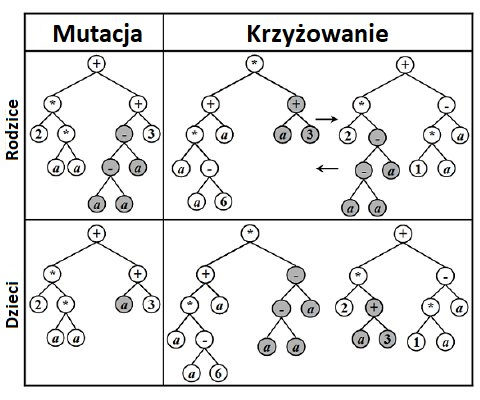
\includegraphics[scale=0.6]{Mutation-and-crossover-operations.jpg}}
	\caption{\label{fig:mutation-and-crossover-operations}Mutacja i krzyżowanie \cite{memetic}}
\end{figure}

Operatory te nie muszą i zazwyczaj nie są stosowane do każdego osobnika w populacji, a to jak często powinny być stosowane, ustalane jest za pomocą odpowiedniego parametru. Zdarza się, że mutacja jest stosowana więcej niż dla danego genu w danym genotypie.

Najczęściej używane operatory krzyżowania to:
\begin{itemize}
\item[•] Krzyżowanie punktowe -- spośród dwóch genotypów losowo wybierany jest jeden punkt, następnie tworzone są dwa nowe genotypy pierwszy z genów na prawo od punktu w pierwszym genotypie i~na lewo w genotypie drugim oraz drugi z dwóch pozostałych.

\item[•] Krzyżowanie dwupunktowe -- spośród dwóch genotypów losowo wybierane są dwa punkty, następnie część pomiędzy tymi punktami jest zamieniana pomiędzy genotypami.

\item[•] Krzyżowanie n-punktowe -- uogólnienie powyższych krzyżowań dla n punktów.

\item[•] Krzyżowanie zamiana w drzewie -- metoda opiera się na modyfikacjach w fenotypie, który jest reprezentowany jako drzewo, w tej metodzie zamieniane są ze sobą dwa poddrzewa. W tym przypadku tworzone są tylko prawidłowe rozwiązania, jednak jest to metoda wymagająca większej ilości obliczeń.  
\end{itemize}
Ponadto krzyżowania możemy podzielić na stało-punktowe, czyli takie, w którym wybierany jest ten sam punktu lub punkty w obu osobnikach, przez co nowe genotypy mieć tę samą długość jak rodzice i~zmienno-punktowe, gdzie mogą to być różne punkty, co skutkuje dużą zmiennością w rozmiarach utworzonych genotypów. 

Natomiast operatory mutacji to:
\begin{itemize}
\item[•] Mutacja punkowa -- dowolny gen w genotypie zostaje zmieniony na inną losową wartość.

\item[•] Mutacja zamiana w drzewie -- metoda opiera się modyfikacjach w fenotypie, który jest reprezentowany jako drzewo, w tej metodzie tworzone jest nowe poddrzewo. Analogicznie jak w przypadku krzyżowania tworzone są tylko prawidłowe rozwiązania, jednak konieczna jest większa ilość obliczeń. 
\end{itemize}

Ostatnim krokiem jest zastąpienie osobników w poprzedniej populacji przez nowych powstałych na skutek zastosowania wcześniej wspomnianych operatorów. Istnieją dwa podejścia: sugerujące zastępowanie całej populacji lub tylko części osobników \cite{SSvsGen}.


\subsection{Ewolucja gramatyczna}
Optymalny model procesu biznesowego może mieć różną wielkość, dlatego chcąc go znaleźć, potrzebna jest metoda, która pozwoli na generowanie rozwiązań o zmiennym rozmiarze. Tradycyjne algorytmy genetyczne operują na stałej strukturze i mogą być użyte na przykład, żeby dobrać odpowiednie parametry do istniejącego modelu. W wielu problemach jednak pożądane jest rozwiązanie o nieznanym rozmiarze, dlatego obecnie najpopularniejsza metoda z tej dziedziny to programowanie genetyczne \cite{Koza:1990:pat-GAsp, 10.5555/138936}, które pozwala na generowanie rozwiązań o różnej długości, dzięki ewolucji całej struktury fenotypu, najczęściej reprezentowanego jako drzewo. Otrzymane rozwiązania są najczęściej gotowymi wykonywalnymi programami, jednak mogą być też równaniami czy modelami.

Na programowaniu genetycznym oparta jest ewolucja gramatyczna \cite{ryan_collins_neill_1998}. Korzysta ona ze standardowych metod ewolucji genetycznej, jednak ewoluuje gramatykę w celu znalezienia programu, który najlepiej rozwiązuje problem. Gramatyka najczęściej zapisana jest w~notacji BNF (sekcja \ref{sec:BNF}). Dzięki zastosowaniu rekursywnych produkcji możliwe jest tworzenie rozwiązań o różnej długości. 

\subsection{Notacja Backusa-Naura}
\label{sec:BNF}
Gramatyka jest zbiorem zasad opisujących budowę języka. Opisuje syntaktykę języka, czyli sposób łączenia poszczególnych symboli, nie mówiąc nic o znaczeniu poszczególnych słów języka. Odnosi się to także do języków formalnych np. języków programowania. Do opisu takich języków służą gramatyki formalne. Na gramatykę formalną składa się uporządkowana czwórka G = (T,N,P,S), gdzie: 

\begin{itemize}
  \item[•] T -- skończony zbiór symboli terminalnych, czyli stałych, symboli, które nie mogą być zastąpione innym ani podzielone na mniejsze 
  \item[•] N -- skończony zbiór symboli nieterminalnych, czyli zmiennych, symboli, które są modyfikowane przy tworzeniu języka
  \item[•] P -- skończony zbiór produkcji, czyli zasad, przekształceń postaci (N$\cup$T)*N(N$\cup$T)* $\rightarrow$ (N$\cup$T)*, czyli przynajmniej jednego symbolu nieterminalnego w dowolny zbiór symboli terminalnych i~nieterminalnych. Gwizdka oznacza wszystkie możliwe słowa nad alfabetem łącznie ze słowem pustym.
  \item[•] S -- symbol startowy, gdzie S $\in$ N
\end{itemize}

W informatyce szczególnie szeroko stosowane są gramatyki bezkontekstowe. Pozwalają one na pokazanie, w jaki sposób rekurencyjnie tworzony jest język, co jest potrzebne, żeby zrozumieć znaczenie programu. Zaletą jest też ich stosunkowo łatwe parsowanie.
Gramatyka bezkontekstowa jest to gramatyka, w której wszystkie produkcje mają postać:
\begin{center}
	A $\rightarrow$ {$\alpha$},
\end{center}
gdzie A jest to pojedynczy symbol nieterminalny -- A $\in$ N, a $\alpha$ to dowolny (także pusty) zbiór symboli terminalnych i~nieterminalnych -- $\alpha \in$ (N$\cup$T)*.
	
Notacja Backusa-Naura (\textit{ang. Backus-Naur Form}) \cite{Backus1959TheSA, Naur, Knuth1964} jest najpopularniejszą notacją używaną do kodowania gramatyk bezkontekstowych. Symbole, które składają się na BNF to:

\begin{itemize}
  \item[•] ::= -- produkcja,
  \item[•] |   -- lub,
  \item[•] <>  -- symbole nieterminalne.
\end{itemize}

Używając tych symboli, możemy opisywać składnię języka w następujący sposób:
\begin{center}
<Nieterminalny1> ::= <Nieterminalny2>Terminalny1 | <Nieterminalny3> | Terminalny1
\end{center}
Oczywiście możliwe jest też definiowanie rekurencyjnie, co pozwala na tworzenie skomplikowanego języka za pomocą prostych zasad: 
\begin{center}
<Nieterminalny1> ::= <Nieterminalny2> | <Nieterminalny2><Nieterminalny1>
\end{center}

\subsection{Tworzenie gramatyki pod kątem ewolucji}
\label{grammarCreation}
Dla każdego problemu można stworzyć nieskończoną ilość poprawnych gramatyk, jednak nie wszystkie z nich będą odpowiednie do zastosowania w algorytmie ewolucji gramatycznej. Chcąc stworzyć gramatykę, która umożliwi najwydajniejsze rozwiązanie problemu można przyjąć kilka wytycznych~\cite{grammarDesign}: 
\begin{itemize}
  \item[•] Każda rekursywna produkcja powinna mieć co najmniej tyle samo produkcji nierekursywnych, inaczej biorąc pod uwagę, że genotyp jest mapowany na fenotyp metodą pseudolosową, prawdopodobieństwo otrzymania rozwiązania, które musi się składać tylko symboli terminalnych, będzie zbyt niskie.
  \item[•] Tworząc gramatykę pod kątem wykorzystania jej w procesie ewolucji, ważne jest, żeby ilość produkcji jak najlepiej odzwierciedlała, jak często chcemy uzyskać dane rozwiązanie.
  \item[•] Stosując mutacje oraz krzyżowanie punktowe lub n-punktowe, które podmienia geny w genotypie, może dojść do sytuacji, w której dany gen po podmianie zostanie zmapowany na produkcje o innej ilości symboli nieterminalnych, przez co kolejne geny, będą mapowane niezgodnie z pierwotnym sensem, gdyż liczba genów w genomie pozostaje stała. Żeby temu zapobiec, należy ograniczyć liczbę symboli nieterminalnych do minimum, a każdy symbol nieterminalny powinien mieć produkcje tworzące tyle samo symboli nieterminalnych oraz możliwie tyle samo produkcji, dzięki czemu po zmapowaniu symbole nadal będą odpowiadały pierwotnym. 
  \item[•] Stworzona gramatyka powinna umożliwić tworzenie jak najmniejszej ilości rozwiązań, które nie należą do języka, co prawda nie uniemożliwi to działania algorytmu, gdyż można odrzucić te rozwiązania na etapie parsowania, ale warto oszczędzić niepotrzebnych obliczeń i rozwiązać ten problem już na etapie tworzenia gramatyki. 
\end{itemize}

\subsection{Omówienia działania algorytmu ewolucji gramatycznej}
Mechanizmem, który wyróżnia ewolucję gramatyczną na tle innych algorytmów ewolucyjnych, jest mapowanie genotypu zapisywanego jako jednowymiarowa tablica liczb całkowitych na fenotyp -- język, zgodnie z zasadami stworzonej gramatyki. Przykładem może być genotyp: 
\begin{center} [6, 71, 92, 59, 52, 95, 23, 45, 12, 2] \end{center}
i gramatyka w notacji BNF:

 \begin{center}
  \begin{tabular}{l}
    \textit{<e> ::= <var>=<math><var>} \\
	\textit{<math> ::= <math><math> | <var><op>} \\
	\textit{<op> ::= + | -} \\
	\textit{<var> ::= a | b | c | d,}
  \end{tabular}
 \end{center}

której symbolem startowym jest <e>. 
Wybór kolejnych produkcji odbywa się według zasady:
\begin{center} $produckja = gen\_jako\_liczba\_całkowita\ \%\ ilosc\_dostepnych\_produkcji$ \end{center}
Używając wyprowadzenia lewostronnego:

\begin{itemize}
  \item[•] Aktualne wyrażenie: <e>; \newline
Aktualny symbol nieterminalny: <e>; \newline
Ilość możliwych produkcji: 1; \newline
Wartość genu: 6; \newline
6 mod 1 = 0, więc <e> zostaje zastąpiony przez <var>=<math><var>
  \item[•] Aktualne wyrażenie: <var>=<math><var>; \newline
Aktualny symbol nieterminalny: <var>; \newline
Ilość możliwych produkcji: 4; \newline
Wartość genu: 71; \newline
71 mod 4 = 3, więc <var> zostaje zastąpiony przez d
  \item[•] Aktualne wyrażenie: d=<math><var>; \newline
Aktualny symbol nieterminalny: <math>; \newline
Ilość możliwych produkcji: 2; \newline
Wartość genu: 92; \newline
92 mod 2 = 0, więc <math> zostaje zastąpiony <math><math>
  \item[•] Aktualne wyrażenie: d=<math><math><var>; \newline
Aktualny symbol nieterminalny: <math>; \newline
Ilość możliwych produkcji: 2; \newline
Wartość genu: 59; \newline
59 mod 2 = 1, więc <math> zostaje zastąpiony <var><op>
\end{itemize}
Kontynuując analogicznie, po zastąpienie wszystkich symboli nieterminalnych, ostatecznie otrzymany fenotyp to:
\begin{center} d = a - b + c \end{center}	
Używając tego prostego mechanizmu, w przypadku bardziej skomplikowanej gramatyki, możliwe jest generowanie znaczniej bardziej złożonych rozwiązań. W połączeniu z metodami z algorytmów ewolucyjnych możliwe jest teoretycznie ewoluowanie programów w dowolnym języku programowania, a następnie za pomocą odpowiedniej funkcji dopasowania znalezienie takiego, który rozwiąże dany problem. W kolejnej sekcji omówiono jak dobrać metryki, aby użyć tego mechanizmu do odkrywania procesów biznesowych.


%---------------------------------------------------------------------------

\section{Metryki}
\label{sec:metryki}

\subsection{Metryki a funkcja dopasowania}

Funkcja dopasowania jest obliczana w każdej iteracji, dla każdego osobnika w populacji, dlatego powinna być możliwie najmniej kosztowna obliczeniowo. Nie warto więc nadmiernie jej komplikować, gdyż nawet jeśli taka wersja lepiej określi, jak dobre jest dane rozwiązanie, to jej obliczenie może stać się wąskim gardłem całego algorytmu, co zwiększy czas potrzebny na znalezienie rozwiązania i pogorszy jego działanie. 

Dobierając funkcję dopasowania, ważne jest, żeby była ona regularna, gdyż duża ilość lokalnych ekstremów może spowolnić ewolucję, a nawet całkowicie uniemożliwić znalezienie globalnie najlepszego rozwiązania.
Nie może więc ona jedynie bezwzględnie mierzyć, jak dobre jest rozwiązanie. Dobrym przykładem jest tutaj problem układanie planów (\textit ang. timetabling problem), gdzie większość otrzymanych rozwiązań będzie nieprawidłowa, a wartość funkcji dopasowania będzie wynosiła zero, nawet jeśli mała zmiana może sprawić, że znalezione zostanie właściwe rozwiązanie, dlatego konieczne jest, jak najlepsze uchwycenie jak blisko algorytm jest prawidłowego rozwiązania \cite{icga85:cramer, beasley:1993:ogapf}.

Ostatecznie funkcja dopasowania w naszym algorytmie jest średnią ważoną metryk wymienionych w sekcji \ref{sec:discovery}, jednak oprócz tego dodano kolejną metrykę złożoność, która ma poprawiać funkcje dopasowania zgodnie z powyższymi zasadami. Użytkownik może określić, z jakimi wagami wziąć pod uwagę poszczególne metryki.

\subsection{Dodatkowa metryka -- złożoność}
\label{sec:additional-metric-complexity}
Dodatkowa metryka zawiera informacje niedotyczące bezpośrednio jakości odkrytego modelu. Istnieją jednak  teoretyczne przesłanki, że powinna wpłynąć pozytywnie na działanie algorytmu. W odróżnieniu od innych metryk celem jej używania jest poprawa wydajności algorytmu ewolucji i próba zminimalizowania czasu potrzebnego na znalezienie rozwiązania.
 
Zamysłem jest promowanie rozwiązywania prostych problemów w prosty sposób i unikanie lokalnych ekstremów -- w tym wypadku sytuacji, w której populacja zostanie zdominowana przez zbyt skomplikowane osobniki na wczesnym etapie ewolucji, zamiast tego ewolucja jest bardziej nakierowana na znajdowanie coraz lepszego rozwiązania wraz ze wzrostem skomplikowania modelu. Analogię można odnaleźć w naturze, w pewnym momencie na Ziemii dinozaury były najlepiej przystosowanymi do życia na tej planecie organizmami -- lokalne maksimum i blokowały powstawanie mniej skomplikowanych form życia, jednak jak pokazuje historia, po wyginięciu dinozaurów, te były w stanie stać się jeszcze lepiej przystosowanymi istotami.

Metryka korzysta z istniejących już obliczeń, przez co nie zwiększa w istotny sposób czasu każdej iteracji algorytmu. Większa złożoność każdego modelu przekłada się także na dłuższe obliczanie pozostałych metryk dla niego, przez co znalezienie ostatecznego rozwiązania zajmuje więcej czasu.


\subsection{Opis i wzory użytych metryk}
\label{sec:metrics-details}
\subsubsection{Prostota}  
Celem używania tej metryki jest zmniejszenie skomplikowania modelu. Głównym czynnikiem na to wpływającym jest liczba aktywności w modelu. Idealna byłaby sytuacja, w której model ma tyle samo aktywności, ile unikalnych aktywności jest w dzienniku zdarzeń. To nie zawsze jest możliwe, jednak chcąc otrzymać maksymalnie czytelny model, powinniśmy do tego dążyć. Stąd też wybrana metryka skupia się na dwóch czynnikach, czyli liczbie duplikatów w modelu i liczbie brakujących wartości w~modelu. Znaczenie ma wielkość modelu, dlatego wartości te muszą zostać odniesione do ilości wszystkich zdarzeń w logu i modelu. Metrykę zapożyczono~z~\cite{qd-in-discovery} i~wyrażono wzorem: \begin{center}
$M_{pro} = 1 - \frac{ilosc\ duplikatow\ w\ modelu\ +\ ilosc\ brakujacych\ zdarzen\ w\ modelu}{ilosc\ unikalnych\ zdarzen\ w\ logu\ +\ ilosc\ zdarzen\ w\ modelu}$
\end{center}
\subsubsection{Odwzorowanie} 
Jest to najbardziej kosztowna obliczeniowo metryka. Pozostałe metryki obliczane są na podstawie informacji uzyskanych podczas jej obliczania. Ważne jest, żeby obliczać odwzorowanie częściowo dla każdej aktywności, a nie całego wariantu procesu, co sprawi, że metryka będzie bardziej wrażliwa na zmiany. Możliwe jest zastosowanie prostej zero-jedynkowej metryki do obliczania, która weryfikowałaby czy model całkowicie zgadza się z wariantem logu, jednak co jest szczególnie niekorzystne w~przypadku algorytmu genetycznego, nie byłoby sprawdzane, o ile bliżej jesteśmy do celu, dopóki losowo nie zostałby znaleziony model idealnie pasujący do wariantu. Metrykę oparto o \cite{metric-calculation}, jednak przy procesie z wieloma aktywnościami, najczęściej duża część aktywności może zostać dopasowana, co sprawi, że łączny błąd będzie niewielki, dlatego wprowadzono modyfikację i podniesiono otrzymany wynik do potęgi 4, żeby zrobić metrykę bardziej wrażliwą na zmiany. Ostatecznie metrykę wyrażono wzorem:
\begin{center}
\begin{tabular}{l}
$M_o = (1 - blad\_odwzorowania)^4$ \\
$blad\_odwzorowania = \frac{\sum_{ilosc\ procesow\ w\ logu} \frac{blad\ odwzorowania\ logu\ w\ modelu}{minimalna\ długosc\ najlepszej\ sciezki\ w\ modelu\ +\ długosc\ sciezki\ w\ logu}}{ilosc\ zdarzen \ w\ logu}$
\end{tabular}
\end{center}
\subsubsection{Precyzja} 
Pozwala na unikanie niewystarczającego dopasowania (\textit{ang. underfitting}). Celem jest uniknięcie tworzenia modeli, według których możliwe są praktycznie dowolne zachowania. Możliwe jest osiągnięcie maksymalnej wartości pozostałych metryk, tworząc bramkę LUB -- OR zawierającą wszystkie aktywności, jednak nie jest to pożądany model. We wzorze skupiono się na ilości osiągalnych zdarzeń następujących po danej aktywności, możliwych w modelu. Chcemy, żeby poszczególne aktywności mogły poprzedzać tylko te, które rzeczywiście poprzedzają w logu. Metrykę oparto o \cite{precision-calculation}, jednak otrzymany wynik podniesiono do potęgi $\frac{1}{3}$, bo oryginalna metryka jest zbyt wrażliwa na zmiany, przez co jest nieproporcjonalna do innych, co zwiększa prawdopodobieństwo utknięcia w lokalnym maksimum, gdzie każda mała zmiana w modelu będzie powodować ogromną zmianę w metryce. Ostatecznie wyrażono ją wzorem:
\begin{center}
$M_{pre} = (1 - \sum_{zdarzenia\ w\ modelu} \frac{ilosc\ osiagalnych\ zdarzen\ w\ modelu\ -\ ilosc\ osiagalnych\ zdarzen\ w\ logu}{ilosc\ osiagalnych\ zdarzen\ w\ modelu})^{\frac{1}{3}} $
\end{center}
\subsubsection{Generalizacja}
Pozwala na unikanie nadmiernego dopasowania (\textit{ang. overfitting}). W pierwszej chwili może wydawać się przeciwieństwem precyzji, jednak chodzi tutaj o uwzględnienie brakujących w dzienniku zdarzeń wariantów, a nie o rozszerzenie modelu o nowe, zupełnie niezwiązane z istniejącymi. Dobrą wizualizacją jej działania jest operacja domknięcia znana z dziedziny przetwarzania obrazów cyfrowych. Generalizację można zmierzyć poprzez obliczenie średniej ważonej liczby przejść w modelu przez dane zdarzenie, dzięki czemu wciąż uwzględniane są ścieżki, które są często odwiedzane w innych wariantach, mimo że pozwalają na zachowanie niewidoczne w dzienniku zdarzeń, a jednocześnie karane jest istnienie ścieżek, które zupełnie nie pokrywają się z żadnymi wariantami. Wraz ze zwiększaniem ilości wykonań danej aktywności wzrasta pewność, że ścieżki ją uwzględniające faktycznie istnieją i ta informacja staje się mniej cenna, dlatego wzięto pierwiastek z liczby wystąpień danego zdarzenia. Metrykę zapożyczono z \cite{qd-in-discovery} i~ostatecznie wyrażono wzorem:
\begin{center}
$M_g = 1 - \frac{\sum_{zdarzenia\ w\ modelu} \frac{1}{\sqrt{ilosc\ wystapien\ zdarzenia}}}{ilosc\ zdarzen\ w\ logu} $
\end{center}
\subsubsection{Złożoność}
Metryka jest powiązana z odwzorowaniem. Jeśli ono rośnie, pozwala się na tworzenie bardziej złożonego modelu. Złożoność jest wyrażana jako ilość wszystkich możliwych ścieżek w modelu. W przypadku pętli jej wartość byłaby nieskończona, dlatego przyjęto, że pętla oznacza maksymalnie dwukrotne jej wykonanie. Jako że np. dla bramki AND jest to n!, zauważamy, że złożoność rośnie niewspółmiernie szybciej do odwzorowania, dlatego we wzorze wzięto pierwiastek z jej wartości. Ostatecznie metrykę wyrażono wzorem: 
\begin{center}
$M_z = 1 - \frac{1}{\sqrt{1\ +\ blad\_odwzorowania\ *\ \sqrt{zlozonosc\ modelu}}} $
\end{center}
\subsection{Obliczanie metryk}
W sekcji \ref{sec:event_logs} przedstawiono przykład dziennika zdarzeń i warianty procesu uzyskane dla niego. Na rys. \ref{fig:metrics_business_process} przedstawiono, jak mógłby wyglądać model tego procesu -- na czerwono zaznaczono ilość wykonań danej aktywności -- oraz zademonstrowano obliczanie metryk:
\newline

\begin{figure}[h]
	\centering{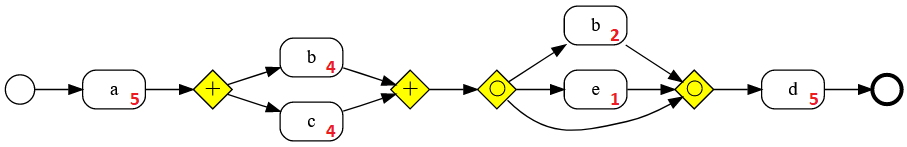
\includegraphics[scale=0.6]{model-metrics-new.png}}
	\caption{\label{fig:metrics_business_process}Model, dla którego obliczane są metryki}
\end{figure}

\subsubsection{Obliczanie prostoty}
Model posiada jeden duplikat -- \textbf{b} oraz jedno brakujące zdarzenie -- \textbf{f}, więc wartość metryki wynosi:
\begin{center}
$M_{pro} = 1 - \frac{1\ +\ 1}{6\ +\ 6} = 0.8333$
\end{center}

\subsubsection{Obliczanie odwzorowania}
\label{sec:alignment-calculation}
Są trzy możliwość na niezgodności modelu z logiem -- brak zdarzenia w modelu, brak zdarzenia w~logu lub zdarzenie w logu różne od zdarzenia w modelu, co może być utożsamiane z brakiem zdarzenia w logu i modelu, dlatego w takim przypadku błąd wynosi 2, a w pozostałych 1. W powyższym przykładzie nieprawidłowe odwzorowanie zachodzi tylko dla jednego wariantu, co można przedstawić na kilka sposobów, jednak nie ma to znaczenia i błąd zawsze wynosi 3 (rys. \ref{fig:bad-alignment}).
\newline
\newline
\begin{figure}[H]
	\centering{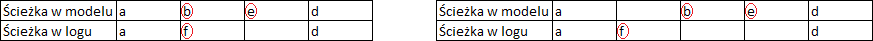
\includegraphics[scale=0.7]{bad-alignment-new.png}}
	\caption{\label{fig:bad-alignment}Nieprawidłowe odwzorowanie}
\end{figure}
Dla pozostałych wariantów odwzorowanie jest pełne i błąd wynosi 0 (rys. \ref{fig:good-alignment}).
\begin{figure}[H]
	\centering{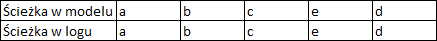
\includegraphics[scale=0.7]{good-alignment.png}}
	\caption{\label{fig:good-alignment}Prawidłowe odwzorowanie}
\end{figure}
Podstawiając wszystkie odwzorowania do wzoru:
\begin{center}
\begin{tabular}{l}
$blad\_odwzorowania = \frac{2 * \frac{0}{5 +\ 5} + \frac{0}{4 +\ 4} + \frac{0}{5 +\ 5} + \frac{3}{4 +\ 3}}{22} = 0.0195$ \\

$M_o = (1 - 0.0195)^4 = 0.9243$
\end{tabular}
\end{center}

\subsubsection{Obliczanie precyzji}
Potrzebna jest ilość osiągalnych, kolejnych zdarzeń dla danej aktywności. Zależy ona od kontekstu, w jakim dana aktywność jest wykonywana np. dla bramki I - AND można jako kolejne wykonać tyle aktywności, ile nie zostało do tej pory wykonanych w tej bramce, z wyjątkiem ostatniej, gdzie przechodzimy do kolejnych aktywności spoza bramki. Dla demonstrowanego przykładu kolejne zdarzenia zaprezentowano na rys. \ref{fig:directly-follows}.
\begin{figure}[H]
	\centering{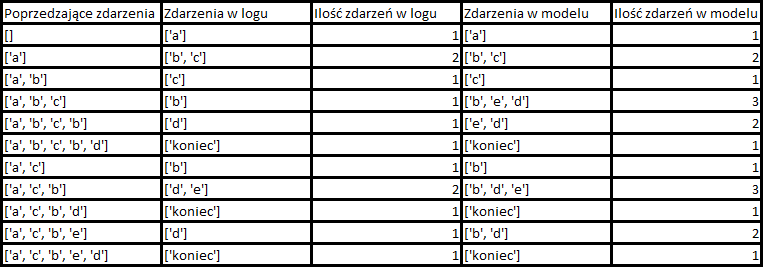
\includegraphics[scale=0.7]{precision-calculation.png}}
	\caption{\label{fig:directly-follows}Kolejne zdarzenia}
\end{figure}
Podstawiając te dane do wzoru:
\begin{center}
$M_{pre} = (1 - (\frac{1\ -\ 1}{1}\ +\ \frac{2\ -\ 2}{2}\ +\ \frac{1\ -\ 1}{1}\ +\ \frac{3\ -\ 1}{3}\ +\ \frac{2\ -\ 1}{2}\ +\ \frac{1\ -\ 1}{1}\ +\ \frac{1\ -\ 1}{1}\ +\ \frac{3\ -\ 2}{3}\ +\ \frac{1\ -\ 1}{1}\ +\ \frac{2\ -\ 1}{2}\ +\ \frac{1\ -\ 1}{1}))^{\frac{1}{3}} = 0.9465 $
\end{center}

\subsubsection{Obliczanie generalizacji}
Jeśli ilość przypadków jest mała, jak w powyższym przykładzie, to generalizacja będzie słaba. W~tym przypadku otrzymano:
\begin{center}
$M_g = 1 - \frac{(\frac{1}{\sqrt{5}}\ +\ \frac{1}{\sqrt{4}}\ +\ \frac{1}{\sqrt{4}}\ +\ \frac{1}{\sqrt{2}}\ +\ \frac{1}{\sqrt{1}}\ +\ \frac{1}{\sqrt{5}})}{6} = 0.3997$
\end{center}

\subsubsection{Obliczanie złożoności}
Złożoność jest obliczana dla poszczególnych bramek logicznych w modelu, co jest konieczne na wcześniejszym etapie działania algorytmu, a następnie te wartości są podstawiane do wzoru wraz z~błędem dopasowania obliczonym w sekcji \ref{sec:alignment-calculation}:\newline
$zlozonosc\_dla\_bramki\_AND = 2! = 2$\newline
$zlozonosc\_dla\_bramki\_OR = 2! * \frac{2!}{(2! * (2 - 2)!)} + 1! *  \frac{2!}{(1! * (2 - 1)!)} + 0! * \frac{2!}{(0! * (2 - 0)!)} = 2 + 2 + 1 = 5$\newline
$zlozonosc = 1 * 2 * 5 * 1 = 10$
\begin{center}
$M_z = 1 - \frac{1}{\sqrt{1 + 0.0195\ *\ \sqrt{10}}} = 0.9706$
\end{center}

\subsubsection{Znaczenie otrzymanych metryk}
Najniższą wartość otrzymano dla generalizacji. Jest to naturalne, gdyż przykładowy dziennik zdarzeń składał się tylko z pięciu przypadków, więc należy spodziewać się nadmiernego dopasowania modelu do logu. Przedstawiony model nie opisuje wszystkich przypadków w modelu stąd niska wartość odwzorowania. Jest on jednak mało złożony i precyzyjny. Możliwe jest znalezienie lepszego modelu, co pokazano w dalszej części pracy.
\chapter{Projekt i implementacja}

\section{Wykorzystane technologie}
\subsection{Python 3.8.1}
Do implementacji algorytmu został użyty Python. Jest to najpopularniejszy język programowania w domenie uczenia maszynowego. Wymagana jest wersja 3.8 lub wyższa ze względu na użycie w implementacji metod dostępnych od tej wersji.  
\subsection{PonyGE2}
PonyGE2 \cite{Fenton_2017} jest implementacją ewolucji genetycznej w języku Python. Pozwala na łatwą konfigurację parametrów ewolucji genetycznej oraz możliwość dodania własnych problemów, a także sposobów ewaluacji rozwiązań. Niestety, PonyGE2 nie jest przystosowane do bycia dołączaną jako niezależna biblioteka i nie umożliwia dostępu poprzez wygodny interfejs.

\begin{figure}[h]
	\centering{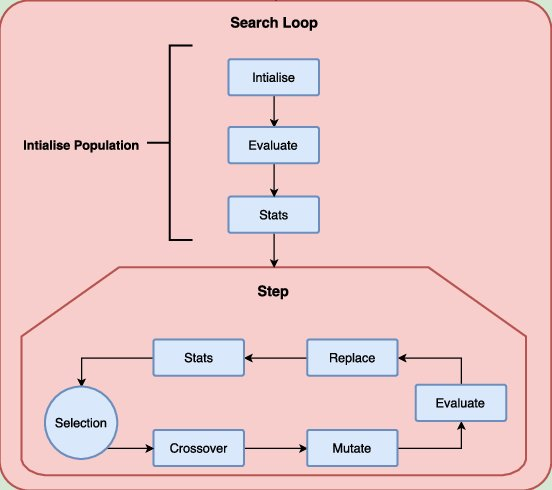
\includegraphics{PonyGE2-search-loop.jpg}}
	\caption{\label{fig:PonyGE2-search-loop}Ogólny schemat działania PonyGE2}
\end{figure}

\section{Tworzenie gramatyki procesu biznesowego}
\label{sec:businessGrammarCreation}
Projektując gramatykę procesu biznesowego, przyjęto dwa początkowe założenia. Uznano, że generowane modele muszą być łatwe do przełożenia na notację BPMN oraz nie powinny być tworzone modele niespójne strukturalnie, co pozwali na zredukowanie przestrzeni rozwiązań, jednocześnie gwarantując tworzenie niegenerujących błędów modeli.

Przy tworzeniu gramatyki procesu biznesowego ważne jest, żeby znaleźć balans, jeśli chodzi o poziom skomplikowania modelu, jaki będzie możliwy do wygenerowania, używając zaproponowanej gramatyki.  W pracy \cite{10.1007/978-3-540-69534-9_35} przeanalizowano składniki języka BPMN pod kątem częstotliwości ich stosowania. Najczęściej używanymi elementami modelów procesu biznesowego, jeśli chodzi o bramki, są: XOR - ALBO kodowane w proponowanej gramatyce jako xor, AND - I jako and oraz pętle jako lo<0$\_$n>. Do przedstawionej dalej gramatyki dodano także bramki OR - LUB reprezentowane jako opt. Ponadto konieczne jest użycie symbolu seq, która oznacza, że aktywności następują kolejno po sobie.

Zgodnie z zaleceniami w sekcji \ref{sec:modelling} przyjmuje się, że dobrą praktyką jest, żeby model zawierał tylko jedno zdarzenie początkowe i końcowe. Z tego powodu przyjęto, że zdarzenia te są domyślnie odpowiednio na początku i końcu wygenerowanego słowa i nie są one jawnie reprezentowane w gramatyce.

W sekcji \ref{grammarCreation} opisano problemem ewolucji gramatyki dla metod opartych o krzyżowanie i mutację punktową lub n-punktową, dlatego zdecydowano się na stworzenie gramatyki pod kątem wersji tych operatorów używających fenotypu - drzewa. Lokalne przeszukiwanie często staje się słabym punktem algorytmów ewolucyjnych. Stosując wspomniane operatory, prawdopodobna jest sytuacja, że mała modyfikacja blisko korzenia może poprawić rozwiązanie, jednak jej zaistnienie wymaga wygenerowania identycznego poddrzewa na nowo, przez co prawdopodobieństwo zaistnienia takiej sytuacji jest niskie. Do rozwiązania tego problemu mogą służyć metody inspirowane algorytmami memetycznymi, a działające na drzewach \cite{memetic}. Dają one możliwość aplikowania lokalnych zmian bez konieczności powtórnego generowania całego poddrzewa, co pozwala na usprawnienie procesu ewolucji. Niestety, użyta biblioteka nie posiada podobnych metod lokalnej optymalizacji. Żeby w pewnym stopniu zaradzić temu problemowi, zmniejszono głębokość potrzebnego do reprezentacji modelu drzewa, jednocześnie zwiększać szanse na lokalne mutacje poprzez wprowadzenie symbolu nieterminalnego <slots>. Sprawia to, że drzewo rośnie bardziej wszerz i oprócz jednego symbolu <anygate>, którego użycie ma zapewnić tworzenie poprawnych, niepustych rozwiązań, generowane są symbole <slot>, które mogą pozostać puste lub wygenerować symbol <anygate> z 10\% prawdopodobieństwem. Przekłada się to na większą ilość lokalnych zmian na późniejszych etapach ewolucji. Lokalne przeszukiwania wspomaga także poprzez reprezentowanie bramki jako dwa odrębne symbole - <name>(<slots>). Dzięki temu w wyprowadzeniu nazwa bramki <name> jest oddzielona on jej zawartości, co sprawia, że możliwa jest zmiana nazwy bramki bez modyfikacji jej wnętrza.

Zaadresowano również konieczność odwzorowania w gramatyce częstotliwości występowania poszczególnych bramek logicznych. Zgodnie z \cite{10.1007/978-3-540-69534-9_35} połączenia i bramki XOR - ALBO, AND - I są tworzone przez większą ilość produkcji niż rzadziej występujące pętle i bramki OR - LUB. 

Zapis GE{\_}RANGE:n jest rozszerzeniem notacji zapewnianym przez PonyGE2, które umożliwia dodanie wygodne dodanie n zmiennych, czyli GE{\_}RANGE:2 w BNF oznacza 0|1|2.
Podobny jest zapis GE{\_}RANGE:dataset{\_}vars, który umożliwia dodanie ilości zmiennych odpowiadającej ich ilości w zbiorze danych w tym wypadku w liczbie aktywności w dzienniku zdarzeń. Został on dodany, dzięki rozszerzeniu standardowego, zapewnianego przez PonyGE2 parsera gramatyki.

Wszystkie bramki mają nazwy tej samej długości - 3 znaki, co ułatwia parsowanie gramatyki. Symbol startowy to <e>.

\begin{figure}[!ht]
\lstset{caption=Proponowana gramatyka procesu biznesowego, captionpos=b}
\lstset{label=src:grammar, frame=single}
\begin{lstlisting}
<e> ::= <slot><slot><anygate><slot><slot>

<anygate> ::=  <anygate><anygate> | <name>(<slots>) | {<event>}

<slot> ::= <anygate> | '' | '' | '' | '' | '' | '' | '' | '' | ''

<slots> ::= <slot><slot><anygate><slot><slot>

<name> ::= and | xor | seq | and | xor | seq | and | xor | seq | 
           and | xor | seq | and | xor | seq | lo<0_n> | lo<0_n> |opt

<event> ::= GE_RANGE:dataset_vars

<0_n> ::= GE_RANGE:5
\end{lstlisting}
\end{figure}

Model, dla którego zaprezentowanie obliczanie metryk (rys. \ref{fig:metrics_business_process}) byłby za pomocą powyższej notacji zakodowany jako:
\begin{center}
(\{a\}and(\{b\}\{c\})opt(\{b\}\{e\})\{d\}
\end{center}

Zapis lo<0$\_$n> jest nieoczywisty, jednak konieczny do reprezentacji pętli, które mogą być przerywane na innej aktywności, niż kończy się ich pojedyncza iteracja.  
Poniższy przykład pokazuje model, który ciężko opisać przy pomocy podstawowych bramek logicznych: 
\begin{figure}[H]
	\centering{\includegraphics[scale=0.4]{grammar-lop-example.png}}
	\caption{\label{fig:subcaption_example}Przykład problemu z pętlą}
\end{figure}
\noindent Jest to możliwe za pomocą słowa - lop oznacza pętle: 
\begin{center}
\{a\}and(\{b\}\{c\})\{d\}lop(\{e\}and(\{b\}\{c\})\{d\})xor(\{f\}\{g\})
\end{center}
Użycie powyższego zapisu jest poprawne, jednak kodowanie pętli w ten sposób sprawia, że powstałe słowo jest skomplikowane, a jego wyewoluowanie mało prawdopodobnie. Problem ten rozwiązano, używając zapisu  lo<0$\_$n>, gdzie <0$\_$n> oznacza, ile znaków ma być pominięte w pierwszej iteracji pętli, dzięki czemu możliwe jest zakodowanie takiej pętli przy użyciu znacznie mniejszej liczb symboli, co ułatwia wyewoluowania takiego modelu. Ten sam model opisany za pomocą stworzonej gramatyki wygląda następująco:

\begin{center}
\{a\}lo1(\{e\}and(\{b\}\{c\})\{d\})xor(\{f\}\{g\})
\end{center}

\section{Projekt systemu}

\subsection{Podział na moduły}

Implementację podzielone na następujące moduły:
\begin{itemize}
  \item[•] wrappers - PonyGE2 nie jest przystosowane do zaimportowania jako biblioteka, dlatego, żeby oddzielić kod PonyGE2 od logiki odkrywania procesów biznesowych, w tym module rozszerzono lub nadpisano cześć z modułów tej biblioteki. Dodano także rozszerzenia do PonyGE2 dodające nowe, brakujące funkcjonalności.
  \item[•] fitness{\_}functions - moduł, w którym znajduje się klasa do obliczania dopasowania, która korzysta z metod w module process{\_}discovery.
  \item[•] process{\_}discovery - moduł zawiera całą logikę parsowania modelu i obliczenia metryk.
\end{itemize}


\begin{figure}[!ht]
	\centering{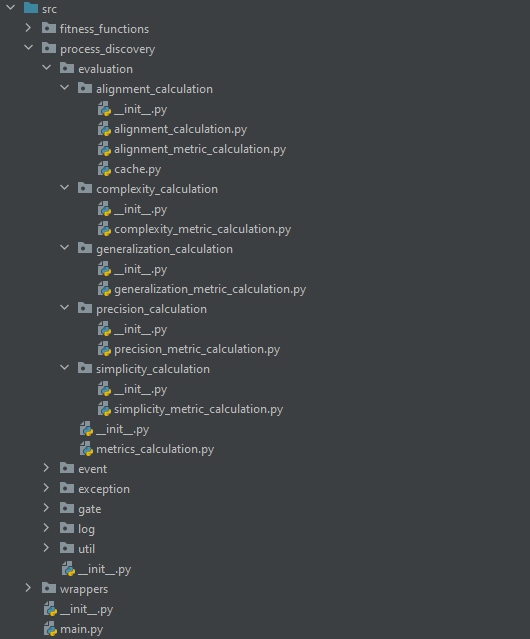
\includegraphics[scale=0.6]{Modules.png}}
	\caption{\label{fig:flow_chart}Podział na moduły}
\end{figure}

\subsection{Model}

Zdecydowano się na podział na dwie reprezentacje modelu procesu biznesowego wykorzystywane na różnym etapie procesowania. Wszystkie klasy implementują interfejs ComparableEvent pozwalający na ich porównywanie definiowanych przez nie obiektów. Aktywności są reprezentowane przez obiekty Event, które przechowują także informacje o ilości przejść w modelu przez dane zdarzenie, potrzebną do obliczenia generalizacji.  

Klasa Gate i klasy po niej dziedziczące są reprezentacją bliższą realnemu modelowi. 

\begin{figure}[h]
	\centering{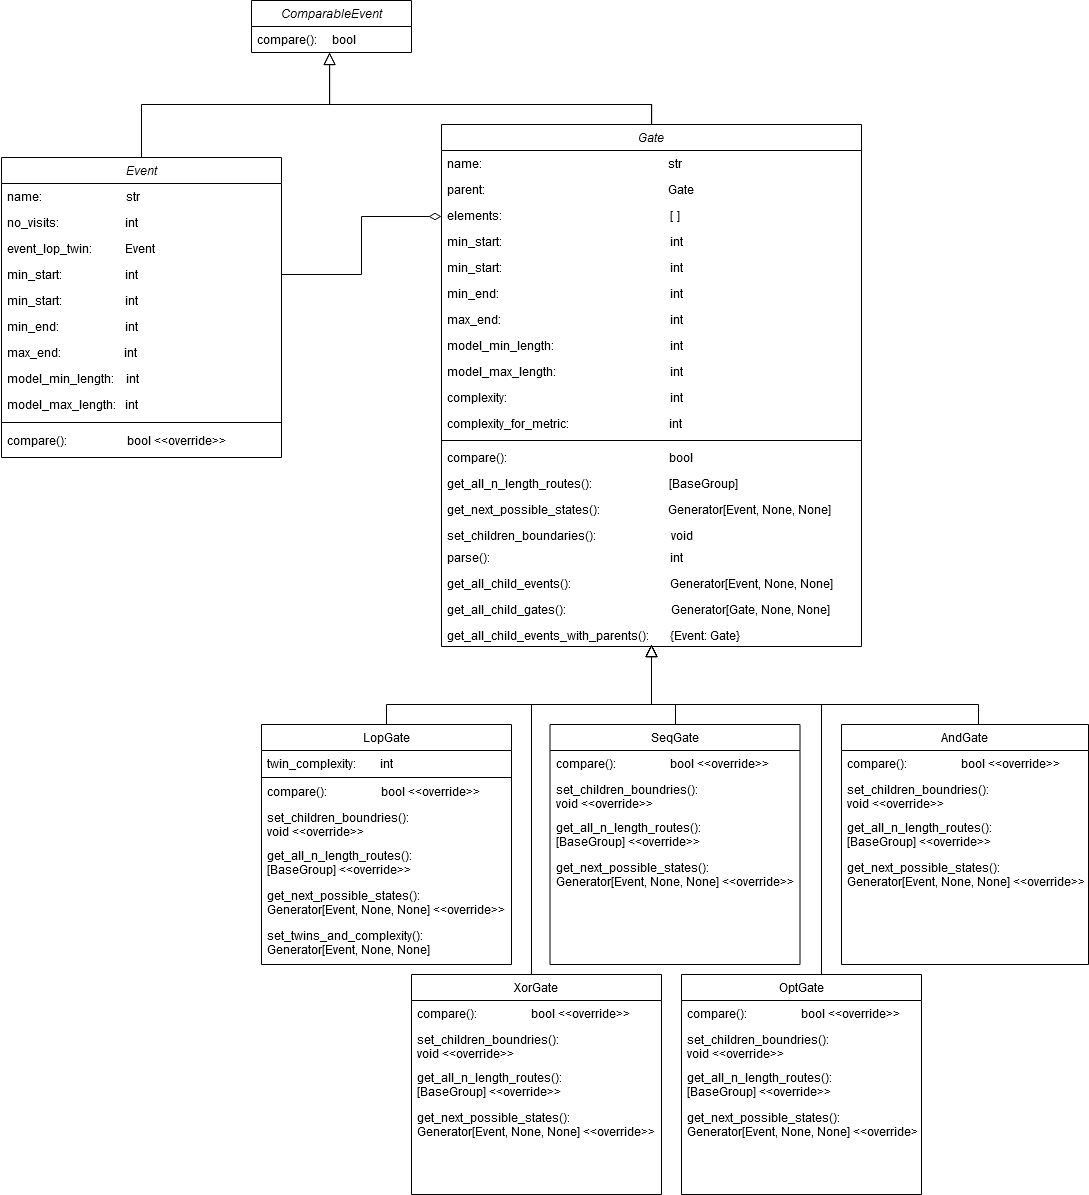
\includegraphics[scale=0.5]{GateUML.png}}
	\caption{\label{fig:subcaption_example}Gate UML}
\end{figure}

Model w formie ciągu znaków musi być zamieniony na formę, na której łatwiej będzie operować. Zakodowane zgodnie z zasadami gramatyki słowo zostaje sparsowane w metodzie parse() klasy Gate na obiekty klas po niej dziedziczących odpowiadające poszczególnym bramką logicznym. Obiekty posiadają wskaźnik na swojego rodzica, czyli bramkę - obiekt Gate, w której się znajduję oraz na bramki lub aktywności - obiekty Event, które zawierają. Przechowują też leniwie obliczaną informacja o złożoności. Najważniejsze metody, które klasy dziedziczące po Gate muszą nadpisać to:
\begin{itemize}
  \item[•] get$\_$next$\_$possible$\_$states() - zwraca jako generator możliwe kolejne aktywności, co jest potrzebne przy liczeniu precyzji.
  \item[•] get$\_$all$\_$n$\_$length$\_$routes() - zwraca możliwe ścieżki w modelu o danej długości jako tablicę obiektów BaseGroup, co jest potrzebne przy liczeniu odwzorowania
\end{itemize}

Obliczanie metryk dla klasy Gate byłoby utrudnione z uwagi na dużą ilość bramek logicznych, dlatego konieczne jest przerobienie tych obiektów na uproszczoną formę pośrednią. Są nią obiekty klas dziedziczących po BaseGroup, które dzielą się pod względem tego, czy aktywności w nich zgrupowane mogą być wykonywane w dowolnej kolejność - EventGroupParallel czy muszą być wykonywane kolejno po sobie - EventGroup. Są to wystarczające informacje do obliczenia dopasowania, a dzięki temu algorytmu ten jest prostszy. Takie rozgraniczenie pozwala również na dodawanie nowych bramek logiczny bez konieczności zmieniana metody obliczanie dopasowania, która jest najbardziej złożonym algorytmem występującym w programie i warto ograniczyć do minimum szansę na konieczność ewentualnych jego modyfikacji. 

\begin{figure}[h]
	\centering{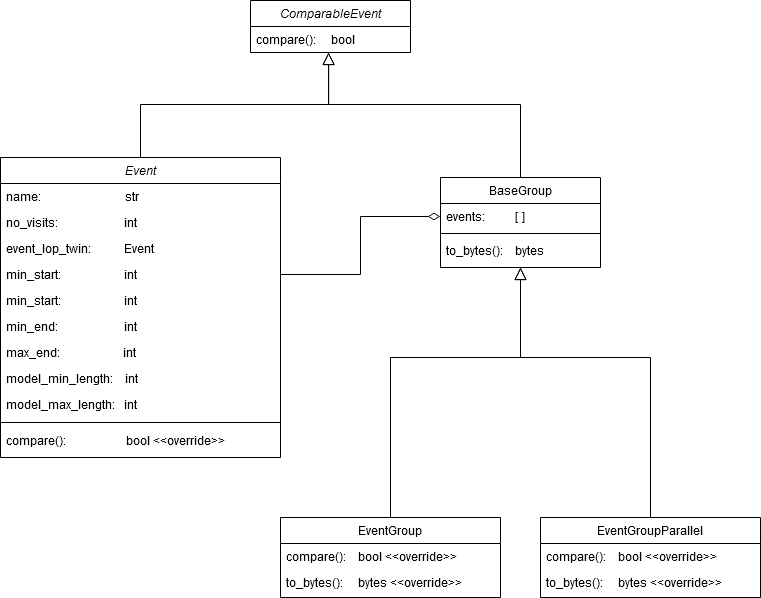
\includegraphics[scale=0.5]{EventUML.png}}
	\caption{\label{fig:subcaption_example}BaseGroup UML}
\end{figure}

Pojedyncze aktywności lub ich grupy są przechowywane jako tablica. Jedyna metoda, która musi zostać nadpisana w klasach rozszerzających BaseGroup to to$\_$bytes() potrzebna przy cachowaniu. 

\section{Implementacja}

W tej części przedstawiono listingi z pseudokodem opartym na języku Python. Tam, gdzie to konieczne pozostawiono słowa kluczowa oraz operatory tego języka.

\subsection{Ogólny schemat blokowy}


\begin{figure}[!ht]
	\centering{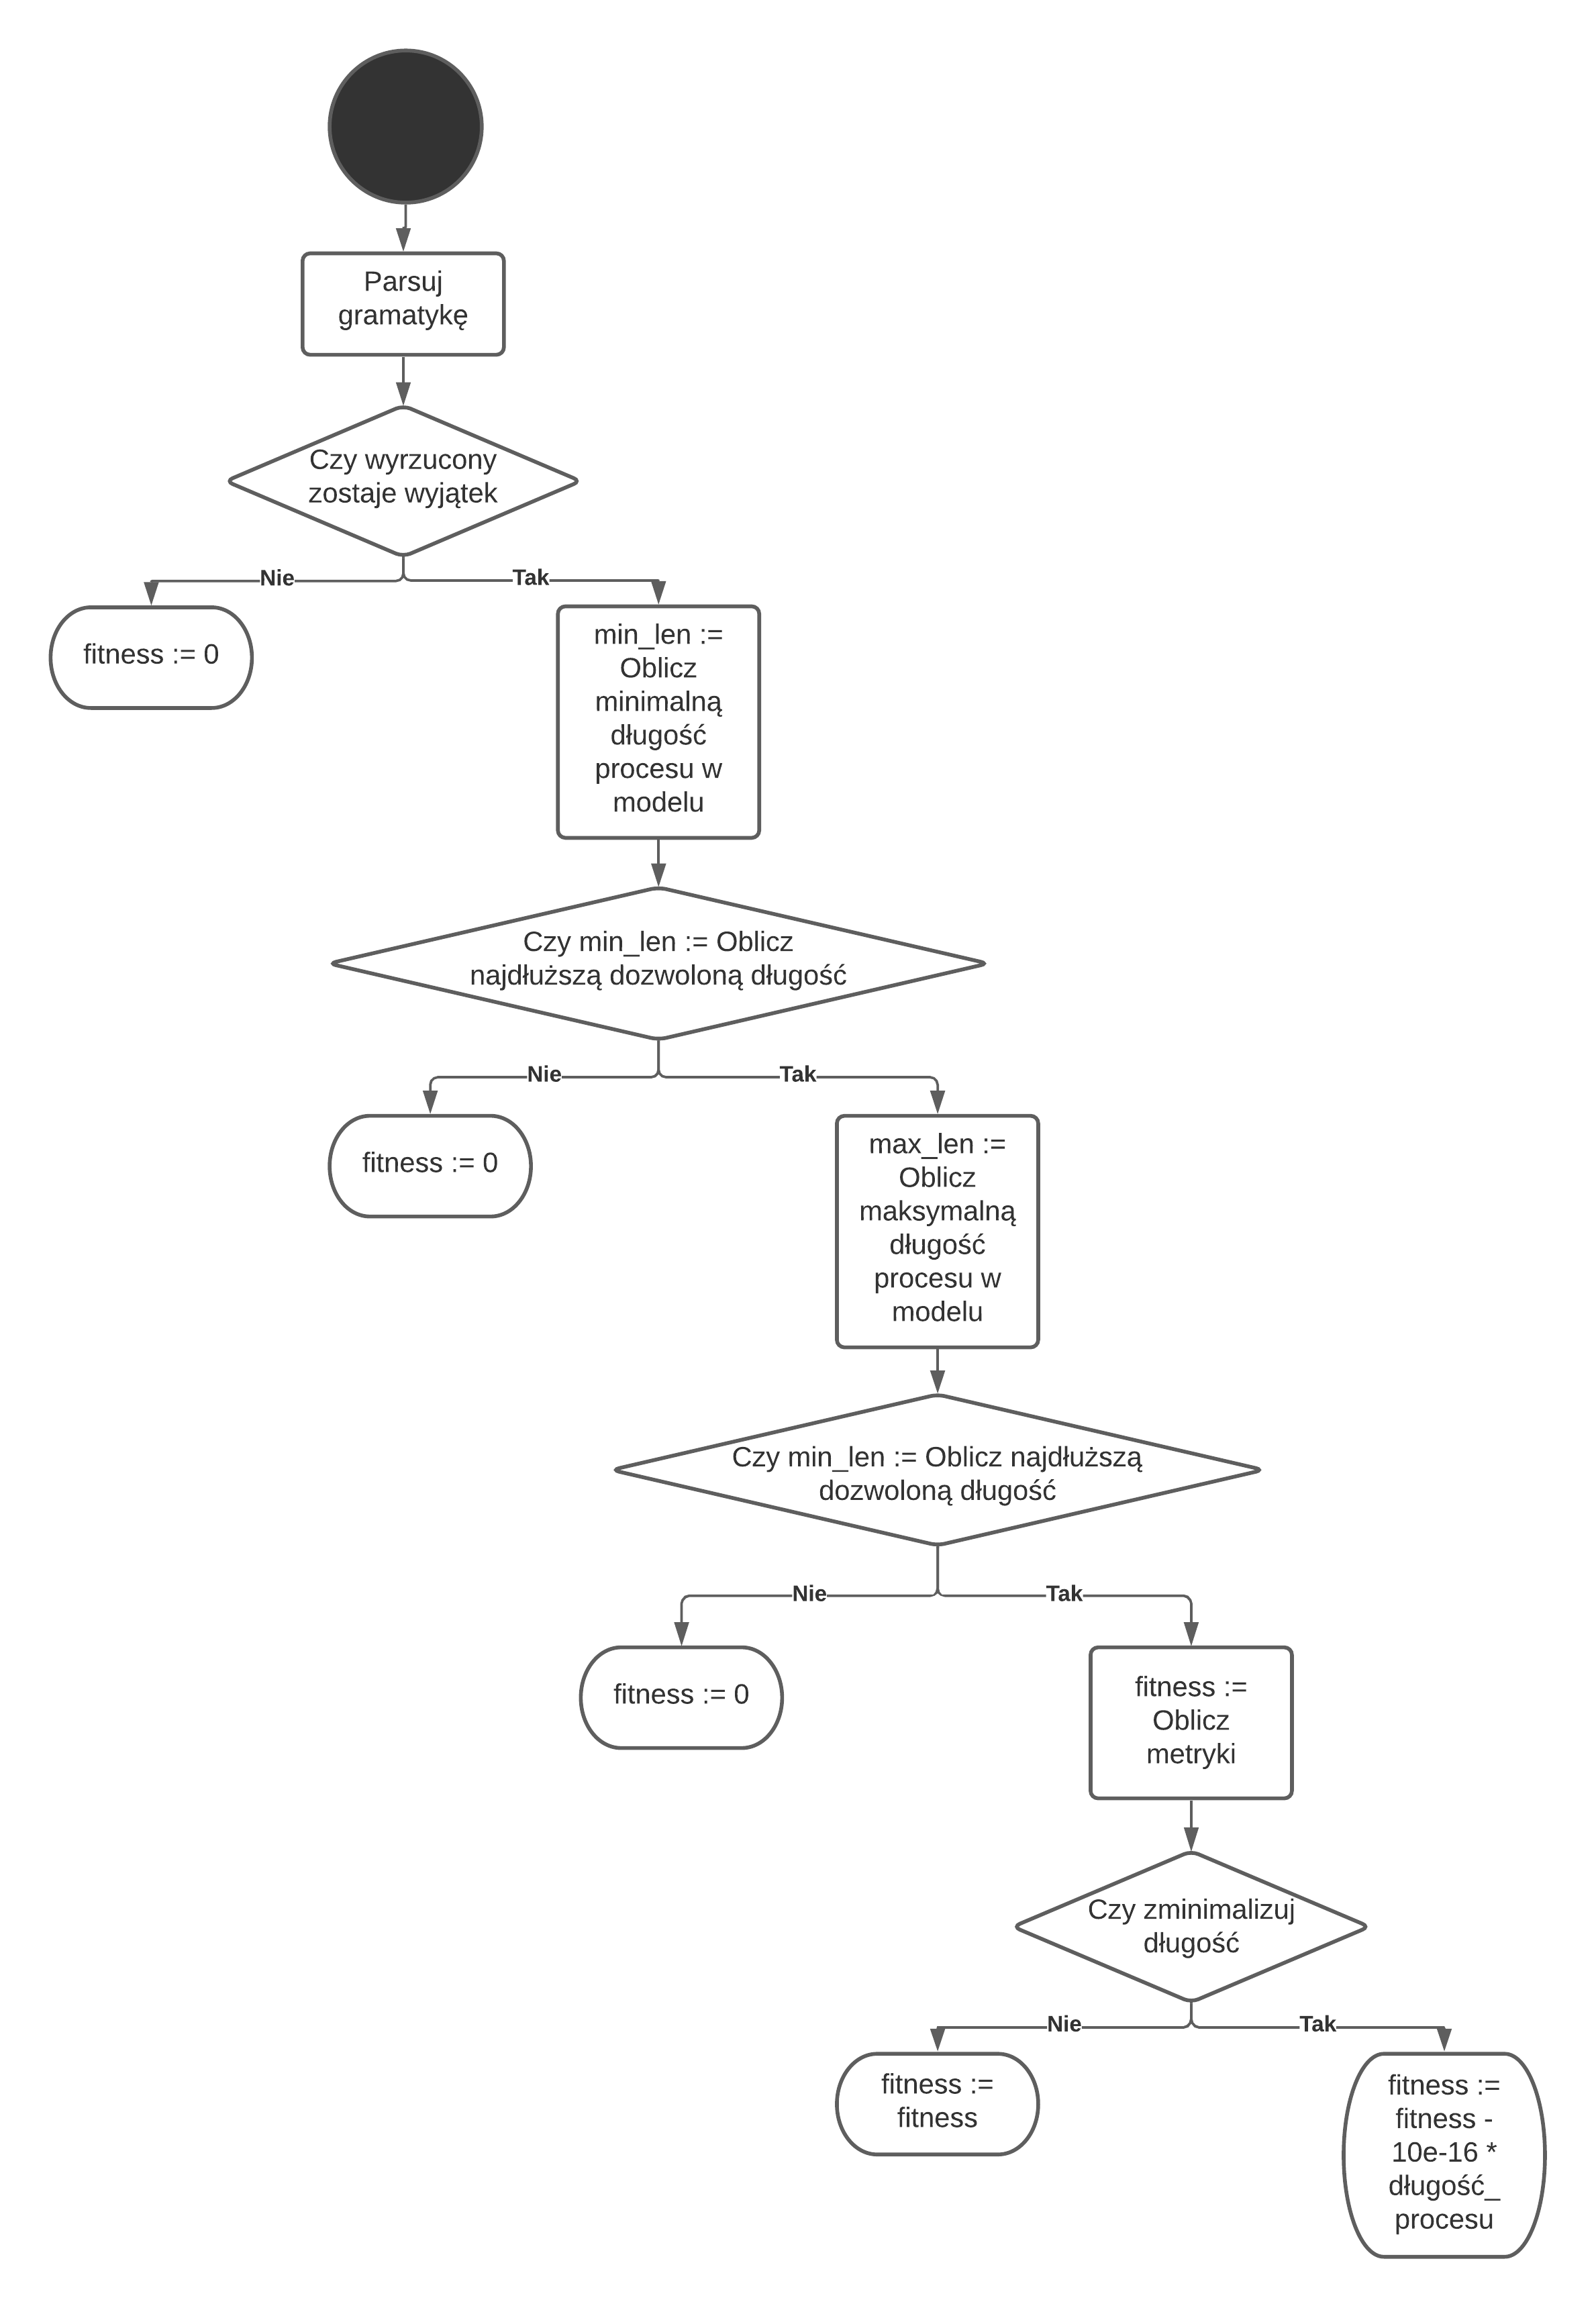
\includegraphics[scale=0.5]{OgolnySchematBlokowy.png}}
	\caption{\label{fig:flow_chart}Ogólny schemat blokowy}
\end{figure}

\subsection{Parsowanie gramatyki}
Parser pozwala na przetworzenie wyników uzyskanych na drodze ewolucji gramatycznej na postać, na której łatwiej będzie operować. Rezultaty uzyskane na drodze ewolucji gramatycznej w PonyGE2 są w formie tekstowej, z którą praca byłaby niewygodna, dlatego używamy parsera, żeby otrzymać wynik w postaci zagnieżdżonych obiektów Gate, które zawierają obiekty Event.

Metoda należy do obiektu Gate i bezpośrednio modyfikuje obiekt, na którym jest wywoływana. Argumentem metody jest wyrażenie wygenerowane w procesie ewolucji. Zwracana jest natomiast ilość przeparsowanych znaków. To na tym etapie odrzucamy też procesy, które, mimo że gramatyka pozwala na ich stworzenie, nie mają sensu z punktu widzenia biznesowego. Pozwala na ograniczenie zbędnego wykorzystania zasobów i niekontynuowanie obliczeń dla modeli, które są bezwartościowe. Są to na przykład procesy, które pozwalają na posiadanie w jednej bramce dwóch takich samych aktywności. Parsując, korzystamy z faktu, że przy projektowaniu gramatyki wszystkie bramki logiczne zostały oznaczone 3-literowymi symbolami, a wszystkie aktywności otoczone są nawiasami klamrowymi. Pasowanie bramek można podzielić na trzy przypadki:
\begin{itemize}   
  \item[•] Bramki ,,seq'' wewnątrz bramek ,,lop'' lub ,,seq'' są redundantne i mogą zostać pominięte.
  \item[•] Pętle ze względu na konieczność specjalnego parsowanie ze względu na problem opisany w sekcji \ref{sec:businessGrammarCreation}.
  \item[•] Pozostałe przypadki.
\end{itemize}


\lstset{caption=Parser gramatyki, captionpos=b}
\lstset{label=src:passive, frame=single}
\begin{lstlisting}[escapeinside=``]
def parsuj(wyrażenie: str) -> int:

   for i in range długość_wyrażenia:
      if wyrażenie[i] == "{":
         zdarzenie := Event(wyrażenia[i + 1])
         dodaj_zdarzenie_do_aktualnie_parsowanej_bramki 
         i += 2
      elif wyrażenie[i] == ")":
         return i+1
      elif i+4 < długość_wyrażenia:
          if wyrażenie[i:i + 3] == "seq" and 
             (self.name == "seq" or self.name == "lop"):
             # pomiń zbędne bramki
             i += 3
             przeparsowane_znaki = bramka.parsuj(wyrażenie[i+4:])
             i += ilość_przeparsowanych_znaków
          else:
             if wyrażenie[i:i+2] == 'lo' and wyrażenie[i:i+3] != 'lop':  
                bramka := stwórz_nową_bramkę_Gate_typu_zgodnego_z_wyrażeniem 
                i += 3
                przeparsowane_znaki = bramka.parsuj(wyrażenie[i+4:])
                if self.name == "seq" or self.name == "lop":
                   if int(wyrażenie[i+2]) <= długość(bramka.elementy):
                      for x in bramka.elementy[int(wyrażenie[i+2]):]:
                         self.dodaj_element(x)
                dodaj_zdarzenie_do_aktualnie_parsowanej_bramki 
                i += ilość_przeparsowanych_znaków
             else:
                bramka := stwórz_nową_bramkę_Gate_typu_zgodnego_z_wyrażeniem 
                i += 3
                przeparsowane_znaki = bramka.parsuj(wyrażenie[i+4:])
                dodaj_zdarzenie_do_aktualnie_parsowanej_bramki 
                i += ilość_przeparsowanych_znaków
       else:
          wyrzuć wyjątek
\end{lstlisting}

\subsection{Obliczanie metryk}
Argumentami metody są obiekt LogInfo zawierający dane i metody dotyczące wariantów, model, czyli obiekt Gate, najkrótsza i najdłuższa dozwolona długość modelu obliczane na podstawie parametru podanego w konfiguracji programu, dzięki czemu możliwe jest zmniejszenie ilości obliczeń oraz cache. Zwracana jest natomiast średnia ważona metryk, czyli wartość funkcji dopasowania. Metryką, która nie wymaga czasochłonnego obliczenia dopasowania, jest prostota, dlatego możemy ją obliczyć wcześniej, co przy niskim wyniku pozwala na wstępne odrzucenie części rezultatów. Łatwo można zauważyć, że jeżeli zdarzenie znajduję się w logu, a nie znajduje się w modelu, dopasowanie nie będzie dobre. Pozwala to przerwać obliczenia, jeżeli stosunek wspólnych zdarzeń w logu i modelu jest mniejszy niż skonfigurowany parametr. Pozostałe metryki wymagają już obliczenia odwzorowania i są obliczane dla najlepiej dopasowanej gramatyki. 

Odwzorowanie obliczane jest osobno dla każdego wariantu w logu, który jest reprezentowany jako tablica znaków. Jeśli błąd dopasowania wynosi 0, to ilość wystąpień danego wariantu konieczna do obliczenia precyzji jest zapisywany w słowniku. Dodawana do każdej aktywności jest też ilość jej dotychczasowych wystąpień potrzebna we wzorze na generalizację.

Po uzyskaniu tych informacji dla wszystkich wariantów obliczamy średnią ważoną metryk zgodnie ze wzorami w sekcji \ref{sec:metrics-details} i uzyskujemy w ten sposób wartość funkcji dopasowania.

\lstset{caption=Obliczanie metryk, captionpos=b}
\lstset{label=src:best_result, frame=single}
\begin{lstlisting}[escapeinside=``]
def oblicz_metryki(log_info, model, najkrótsza_dozwolona_długość, 
                   najdłuższa_dozwolona_długość, cache) -> int:
                   
   lista_zdarzeń_w_modelu = model.zwróć_listę_zdarzeń_w_modelu()
   metryki['PROSTOTA'] := oblicz_metrykę_prostota(lista_zdarzeń_w_modelu, 
                                                  unikalne_zdarzenia_w_logu)
   if metryki['PROSTOTA'] < MINIMALNY_PRÓG_PROSOTY:
      return 0
   stosunek_wspólnych_zdarzeń_w_logu_i_modelu := 
      oblicz_stosunek_wspólnych_zdarzeń_w_logu_i_modelu(lista_zdarzeń_w_modelu, 
                                                        unikalne_zdarzenia_w_logu)		   
      if stosunek_wspólnych_zdarzeń_w_logu_i_modelu <
         MINIMALNY_STOSUNUK_WSPÓLNYCH_ZDARZEŃ_W_LOGU_I_MODELU:
      return stosunek_wspólnych_zdarzeń_w_logu_i_modelu/10
        
   idealnie_dopasowane_logi := pusty_słownik
   skumulowany_błąd := 0
    
   for wariant in log:
      minimalny_błąd_dopasowania,najlepiej_dopasowane_zdarzenia,najlepsza_ścieżka := 
      oblicz_dopasowanie_dla_jednego_wariantu(wariant, model, 
                                              najkrótsza_dozwolona_długość, 
                                              najdłuższa_dozwolona_długość, cache)
      if minimalny_błąd_dopasowania == 0:
         idealnie_dopasowane_logi[najlepiej_dopasowane_zdarzenia] := 
         log_info[wariant].ilość_wystąpień
      dodaj_wystąpienia(lista_zdarzeń_w_modelu, najlepiej_dopasowane_zdarzenia, 
                        log_info[wariant].ilość_wystąpień)

   metryki := oblicz_metryki 
   fitness := oblicz_średnią_ważoną_metryk
   return fitness
\end{lstlisting}

\subsection{Obliczanie dopasowania dla pojedynczego wariantu}
Procedurę obliczenia dopasowana można podzielić następująco:
\begin{itemize}
  \item[•] Znalezienie ścieżek o długości \textbf{n} w modelu.
  \item[•] Przerobienie ścieżek na postać BaseGroup.
  \item[•] Obliczenie dopasowania.
\end{itemize}

Argumentami metody są wariant, model, najkrótsza i najdłuższa dozwolona długość modelu oraz cache. Zwracane są natomiast minimalny błąd dopasowania jako liczba całkowita niedodatnia, najlepiej dopasowane zdarzenia jako tablica obiektów Event oraz najlepsza ścieżka jako obiekt BaseGroup.

Algorytm obliczania dopasowania wymaga ścieżek o stałej, określonej długość. Ważne jest, żeby jak najbardziej ograniczyć czas potrzebny na znalezienie najlepszej ścieżki, dlatego obliczanie dopasowania rozpoczynamy o \textbf{n} równego długości wariantu. Jeśli \textbf{n} jest różne od długości ścieżki, błąd dopasowania zawsze będzie równy przynajmniej różnicy tych wartości. Jednak wciąż może być lepszy niż aktualnie najmniejszy, więc obliczamy dopasowanie kolejno dla ścieżek o długości n-1, n+1, n-2, n+2... aż do momentu, dopóki jest możliwe uzyskanie mniejszego błędu lub zostanie osiągnięty limit, do którego w konfiguracji zezwolono na szukanie. 

Następnie obliczane jest najwcześniejsze i najpóźniejsze wystąpienie danej aktywności w modelu, co ułatwi dalsze obliczenia. W kolejnym kroku znajdowane są wszystkie ścieżki o długości \textbf{n} w modelu i są one sortowane względem procentu wspólnych zdarzeń w modelu i logu. Możemy z tego wywnioskować jakie najlepsze dopasowanie można otrzymać dla danej ścieżki i ewentualnie jeśli przekroczona jest dopuszczalna tolerancja błędu dopasowania lub nie jest możliwe już zmniejszenie błędu przerwanie obliczeń dla niej.    

W końcu zgodnie z kolejnością po sortowaniu obliczane jest dopasowanie i jeśli błąd jest mniejszy niż aktualnie najmniejszy, zamieniane są wartości minimalnego błędu dopasowania, najlepiej dopasowane zdarzenia i najlepsza ścieżka, a jeśli błąd wynosi 0, algorytm jest przerywany i te wartości są zwracane.

\lstset{caption=Obliczanie dopasowania dla jednego wariantu, captionpos=b}
\lstset{label=src:best_result, frame=single}
\begin{lstlisting}
def oblicz_dopasowanie_dla_jednego_wariantu(wariant, model, 
                                            najkrótsza_dozwolona_długość, 
                                            najdłuższa_dozwolona_długość, cache):
   dłogość_wariantu := oblicz_długość(wariantu)
   n := dłogość_wariantu
   i := 1
   minimalny_błąd_dopasowania := -(dłogość_wariantu + model.minimalna_długość)
   najlepiej_dopasowane_zdarzenia := []
   najlepsza_ścieżka := []
   dolny_limit_osiągnięty := False
   górny_limit_osiągnięty := False
   
   while not (dolny_limit_osiągnięty and górny_limit_osiągnięty):
      if n >= min(oblicz_maksymalną_dozwoloną_długość(dłogość_procesu), 
                  dłogość_procesu - minimalny_błąd_dopasowania):
         górny_limit_osiągnięty := True
         n += (-i if i % 2 == 1 else i); i += 1
         continue
      if n <= max(oblicz_minimalną_dozwoloną_długość(dłogość_wariantu), 
                  dłogość_wariantu + minimalny_błąd_dopasowania):
         dolny_limit_osiągnięty := True
         n += (-i if i % 2 == 1 else i); i += 1
         continue
         
      if najkrótsza_dozwolona_długość <= n <= najdłuższa_dozwolona_długość:
         ustaw_najwcześniejsze_i_najpóźniejsze_wystąpienie_zdarzenia(model, n)
         ścieżki = model.znajdź_wszystkie_ścieżki_długości_n(n, wariant)
         if ścieżki istnieją:
            for ścieżka in ścieżki:
               procent_wspólnych_zdarzeń := oblicz_procent_wspólnych_zdarzeń_
                  w_modelu_i_logu(ścieżka, wariant)
               if procent_wspólnych_zdarzeń >= 1 - TOLERANCJA_BŁĘDU_DOPASOWANIA:
                  dodaj sćiezkę do lista_ścieżek_do_obliczenia
            posortowane_ścieżki := posortuj lista_ścieżek_do_obliczenia
            for ścieżka in posortowane_ścieżki:
               if procent_wspólnych_zdarzeń <= 1 + minimalny_błąd_dopasowania /
                  długość_wariantu:
                  break
               błąd_dopasowania, najlepiej_dopasowane_zdarzenia :=
               oblicz_dopasowanie(ścieżka, wariant, cache)
               if błąd_dopasowania > minimalny_błąd_dopasowania:
                  minimalny_błąd_dopasowania := błąd_dopasowania
                  najlepiej_dopasowane_zdarzenia := dopasowane_zdarzenia
                  najlepsza_ścieżka := scieżka
               if błąd_dopasowania == 0:
                  return minimalny_błąd_dopasowania, najlepiej_dopasowane_
                         zdarzenia, najlepsza_ścieżka
      n += (-i if i % 2 == 1 else i); i += 1
   return minimalny_błąd_dopasowania, najlepiej_dopasowane_zdarzenia, 
          najlepsza_ścieżka
\end{lstlisting}

\subsection{Wyszukiwanie w modelu ścieżek o określonej długości}

Łatwiejszym niż obliczenie dopasowania dla modelu składającego się z bramek logicznych jest znalezienie najpierw w modelu wszystkich ścieżek o określonej długości. Algorytm służący do tego jest kolejno wywoływane dla wszystkich bramek - podmodeli, a następnie na podstawie ścieżek znalezionych w podmodelach są tworzone ścieżki dla całego modelu. Implementacja różni się w zależności od przeszukiwanej bramki logicznej. Poniżej zaprezentowano przykład dla bramki ,,and''.  

Argumentami metody długość szukanej ścieżki oraz wariant jako tablica znaków potrzebny wyszukiwanie ścieżek dla obiektu LopGate. Zwracana jest natomiast lista wszystkich ścieżek o określonej długość jako obiekty BaseGroup, a w przypadku błędu None.

Bramki mogą zawierać różną ilość elementów, dlatego należy obliczyć minimalne i maksymalne długości, czyli ilość zdarzeń dla wszystkich dzieci. Jeśli dziecko jest obiektem Event, wtedy dodawane jest bezpośrednio do listy rezultatów. W innym wypadku, kiedy jest obiektem Gate, na podstawie długości dzieci obliczany jest dolny i górny limit długości, dla jakich zostanie dla danego elementu wywołana metoda znajdź{\_}wszystkie{\_}ścieżki{\_}długości{\_}n. Dzięki temu może znacznie ograniczyć ilość długości, dla jakich trzeba przeszukiwać podmodele. Wszystkie znalezione ścieżki są dodawane do listy, a całość do globalnej listy. 

Rezultat nie może być jednak zagnieżdżoną listą, więc musi ona zostać przerobiony na listę jednowymiarową rozwiązań. Każda lista składa się 2-wymiarowej listy ścieżek dla każdego elementów modelu. Ścieżki każdego podmodelu są łączone ze ścieżkami kolejnych podmodeli każda z każdą, żeby utworzyć możliwe przejścia dla całego modelu. Celem jest znalezienie tylko tych o długości \textbf{n}, więc pozostałe odrzucamy. Na końcu, jako że jest to bramka ,,and"" wszystkie ścieżki o długości większej niż 1 są opakowywane w EventGorupParrallel, żeby zachować informacje o tym, ze zdarzenia mogą być wykonywane w dowolnej kolejności.
\clearpage

\lstset{caption=Wyszukiwanie procesów o długości n, captionpos=b}
\lstset{label=src:get_n_length, frame=single}
\begin{lstlisting}[escapeinside=``]
def znajdź_wszystkie_ścieżki_długości_n(n, wariant) -> [BaseGroup]:
   if n == 0:
      return []
   if self.minimalna_długość_modelu < n or n < self.maksymalna_długość_modelu:
      return None

   minimalne_długości := self.oblicz_minimalne_długości_dzieci()
   maksymalne_długości := self.oblicz_maksymalne_długości_dzieci()
   globalna_lista := []

   for element in self.elementy:
      lokalna_lista := []
      if isinstance(element, Event):
         lokalna_lista.dodaj(elem)
         minimalne_długości.usuń_na_pozycji(0)
         maksymalne_długości.usuń_na_pozycji(0)
      else:
         dolny_limit, górny_limit := 
         self.oblicz_docelowy_zakres(n, globalna_lista, minimalne_długości, 
                                     maksymalne_długości)
         for i in range(dolny_limit, górny_limit + 1):
            try:
               wszystkie_ścieżki_dziecka_o_długości_n := 
               element.znajdź_wszystkie_ścieżki_długości_n(i, wariant)
            except ValueError:
               return None
            if wszystkie_ścieżki_dziecka_o_długości_n is not None:
               loklana_lista.dodaj(wszystkie_ścieżki_dziecka_o_długości_n)

         if lokalna_lista:
            globalna_lista.dodaj(lokalna_lista)

   ścieżki = []
   if globalna_lista:
      for element in spłaszcz_listę(globalna_lista):
         if self.sprawdź_długość(n, elem):
            if n == 1:
               ścieżki.dodaj(element[0])
            else:
               ścieżki.dodaj(EventGroupParallel(element))
   if ścieżki:
      return ścieżki
   else:
      return None
\end{lstlisting}

\subsection{Obliczanie dopasowania}
Pomysł zaczerpnięty z algorytmu Needlemann-Wunsch \cite{ea252fd3937a4a309a5e07e61e5531a7}, który jest uogólnieniem odległości Levenshteina dla dowolnych wartości błędów. Tworzymy macierz o wymiarach długość modelu i długość logu, w której obliczana jest najmniejsza suma błędów. Rozwinięty o możliwość przeszukiwania modelu rekurencyjnie oraz o możliwość podawania listy równoległych zdarzeń.

Podstawowy algorytm można opisać za pomocą czterech kroków dla każdego zdarzenia:  
\begin{enumerate}
  \item Oblicz wartość w poprzednim wierszu i kolumnie dodać błąd ,,dopasowanie'' lub ,,brak dopasowania''.
  \item Oblicz wartość w poprzednim wierszu dodać błąd ,,przerwa''.
  \item Oblicz wartość w poprzedniej kolumnie dodać błąd ,,przerwa''.
  \item Wybierz najmniejszą wartość.
\end{enumerate}

\begin{figure}[h]
	\centering{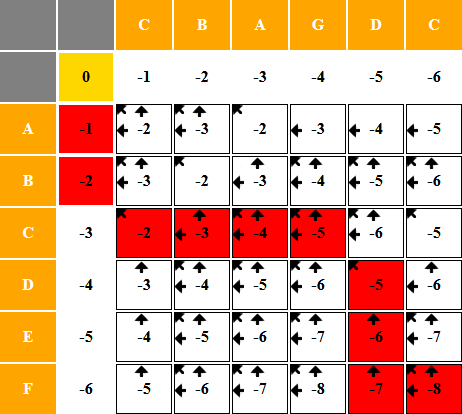
\includegraphics[scale=0.8]{needlemann-wunsch-algo.png}}
	\caption{\label{fig:algo_example}Klasyczny algorytm Needlemann-Wunsch}
\end{figure}


Argumentami metody model jako obiekt Gate oraz wariant jako tablica znaków. Zwracane są natomiast ostatni wiersz, który zawiera błąd dopasowania modelu oraz pośrednie błędy dla wszystkich zawsze zaczynając od pierwszego zdarzenia możliwych długości wariantu, co jest potrzebne, jeśli model zawiera podmodele oraz najlepiej dopasowana ścieżka. Metoda opakowana jest w metodę, która jeśli dla danego modelu i wariantu zostało już obliczone dopasowanie, zwraca rozwiązanie z cache bez powtarzania obliczeń.

Zgodnie z \ref{alignment-calculation} brakujące zdarzenie to błąd wynosi 1, a jeśli się nie zgadzają - 2. Stworzona macierz jest inicjalizowana zerami, a następnie pierwsza kolumna jest wypełniana stosownymi wartościami błędu. Są trzy opcja normalne obliczenie zgodne z klasycznym algorytmem, a także sytuacja, w której model zawiera podmodele, gdzie algorytm jest powtórnie wywoływany dla podmodelu i dla wszystkich zawsze zaczynając od pierwszego zdarzenia możliwych długości wariantu lub gdy zawiera zdarzenia równoległe - EventGroupParallel wtedy stosujemy inny algorytm, który bezpośrednio porównuje wszystkie zdarzenia w wariancie ze zdarzeniami w obiekcie EventGroupParallel. 
     
\lstset{caption=Obliczanie dopasowania, captionpos=b}
\lstset{label=src:alignment_calculation, frame=single}
\begin{lstlisting}[escapeinside=``]
def oblicz_dopasowanie(model, wariant):
   błąd := {'DOPASOWANIE': 0, 'BRAK_DOPASOWANIA': -2, 'PRZERWA': -1}
   ilość_wierszy = długość(model) + 1
   ilość_kolumn = długość(wariant) + 1
   najlepiej_dopasowane_ścieżki_podmodeli := [None] * ilość_wierszy
   macierz_rozwiazań := zainicjalizuj_macierz_zerami()

   for j in range(ilość_kolumn):
      macierz_rozwiązań[0][j] := błąd['PRZERWA'] * j

   for i in range(1, ilość_wierszy):
      if jest_podmodelem(model[i-1]):
         macierz_rozwiązań[i], najlepiej_dopasowane_ścieżki_podmodeli[i] := 
         dopasowanie_podmodeli(macierz_rozwiazań[i - 1], model[i - 1],
                                  [x for x in odwrócone_substringi(wariant)], i)
      elif długość(model[i-1]) > 1:
         macierz_rozwiązań[i], najlepiej_dopasowane_ścieżki_podmodelu[i] := 
         dopasowanie_równoległe(macierz_rozwiazan[i - 1], model[i - 1],
                                [x for x in odwrócone_substringi(wariant)], kara, i)
      else:
         macierz_rozwiazań[i][0] := macierz_rozwiązań[i-1][0] + kara['PRZERWA']
         dopasowanie(macierz_rozwiazań, model[i - 1], wariant, kara, i, ilość_kolumn)

   najlepiej_dopasowana_ścieżka := 
   znajdź_ściezkę(macierz_rozwiązań, błąd['PRZERWA'], model, wariant, 
                  najlepiej_dopasowana_ścieżka_podmodelu)

   return macierz_rozwiązań[ilość_wierszy-1], najlepiej_dopasowana_ścieżka
\end{lstlisting}

\subsection{Znajdowanie najlepiej dopasowanych aktywności w modelu}
Potrzebne do obliczenia precyzji oraz generalizacji. Algorytm obliczanie dopasowania zwraca najmniejszy błąd, ale nie daje informacji o tym, dla jakiej ścieżki otrzymano ten błąd. Dodatkowo Znajdowanie najlepiej dopasowanych aktywności w modelu jest utrudnione przez fakt, że modele może składać się z podmodeli - BaseGroup. 

Argumentami metody są kopia macierzy rozwiązań, model, kopia wariantu oraz rozwiązania podmodeli. Zwracana jest natomiast najlepiej dopasowana ścieżka.

Algorytm zaczyna znajdowanie ścieżki od ostatniego elementu i cofa się do początku. W komórkach, dla których znaleziono dopasowanie, wpisywane jest 0. Tak jak poprzednio, są trzy możliwość brak zdarzenia w modelu, w logu, oraz zupełna niezgodność. Ścieżki szuka się poprzez porównywanie wartości w komórce z suma błędów z wartościami odpowiednich kolumn. Znalezioną ścieżkę pokazano na rysunku \ref{fig:algo_example}. Uwzględnione muszą być dwie sytuacje - taka, w której dana pozycja została obliczona dla podmodelu lub nie.

W tym drugim, jeśli zdarzenie zostało pominięte w modelu, to wpisywane jest do ścieżki None, natomiast jeżeli zostało znalezione dopasowanie, to dodajemy zdarzenie do modelu i usuwamy z wariantu.

Jeśli dana pozycja została obliczona dla podmodelu, algorytm działa podobnie, największą różnicą jest to, że w takiej sytuacji nie ma jednego zdarzenie tylko kilka i tylko część może się zgadzać. Dlatego znajdujemy ostatnie \textbf{k} zdarzeń w podmodelu dla każdego podwariantu i kolejno porównujemy ich ilość i różnicę w błędzie, dzięki czemu dowiemy się, dla którego podwariantu znaleziono najlepsze dopasowanie. 

\lstset{caption=Znajdowanie ścieżki w modelu, captionpos=b}
\lstset{label=src:traceback, frame=single}
\begin{lstlisting}[escapeinside=``]
def znajdź_ścieżkę(macierz_rozwiązań, model, wariant, 
                   rozwiązania_podmodeli) -> [Event]:
   ścieżka = []
   i = długość(model)
   j = długość(wariant) 
    
   while i != 0:
      długość_podmodelu = długość(model[i - 1])
      if rozwiązania_podmodeli[i] is not None:
         znaleziono_dopasowanie := False
         if macierz_rozwiązań[i][j] == 
            macierz_rozwiązań[i - 1][j] + długość_podmodelu * błąd['PRZERWA']:
            [ścieżka.dodaj(None) for _ in range(długość_podmodelu)]
            macierz_rozwiązań[i][j] := 0
            i -= 1
         else:
            for k in range(j):
               zdarzenia := znajdź_nie_none(rozwiązania_podmodeli[i][k])
                            [długość(rozwiązania_podmodeli[i][k]) - (j-k)], wariant)
               if macierz_rozwiązań[i][j] == macierz_rozwiązań[i - 1][k] + 
                  (długość_podmodelu + (j-k) - 2*długość(zdarzenia))*błąd['PRZERWA']:
                  [ścieżka.dodaj(x) for x in odwróć(zdarzenia)]
                  for x in zdarzenia:
                     wariant = wariant.usuń(x.nazwa)
                  [ścieżka.dodaj(None) 
                   for _ in range(długość_podmodelu - długość(zdarzenia))]
                  macierz_rozwiązań[i][j] := 0
                  i -= 1
                  j = k
                  znaleziono_dopasowanie = True
                  break
            if not znaleziono_dopasowanie:
               if macierz_rozwiązań[i][j] == macierz_rozwiązań[i][j - 1] + 
                                             błąd['PRZERWA']:
                  macierz_rozwiązań[i][j] := 0
                  j -= 1
      else:
         if macierz_rozwiązań[i][j] == macierz_rozwiązań[i - 1][j] + kara:
            ścieżka.dodaj(None)
            macierz_rozwiązań[i][j] := 0
            i -= 1
         elif macierz_rozwiązań[i][j] == macierz_rozwiązań[i][j - 1] + kara:
            macierz_rozwiązań[i][j] := 0
            j -= 1
         elif macierz_rozwiązań[i][j] == macierz_rozwiązań[i - 1][j - 1]:
            ścieżka.dodaj(model[i-1])
            wariant = wariant.usuń(model[i-1].nazwa)
            macierz_rozwiązań[i][j] := 0
            i -= 1 
            j -= 1
   return ścieżka
\end{lstlisting}

\subsection{Pozostałe wnioski dotyczące implementacji}
Używając algorytmów genetycznych, konieczne jest wielokrotne obliczenie metryk, żeby znaleźć rozwiązanie. Z tego powodu, duży nacisk na położono na ograniczenie czasu obliczeń. W wiele miejscach zaimplementowano mechanizm przerywający obliczenia, jeżeli nie dają one perspektyw na znalezienie lepszego niż aktualnie najlepsze rozwiązanie. Użytkownik może też zdefiniować maksymalną złożoność modelu, co przełoży się także na czas jego znajdowania. Duże znaczenie ma też fakt, że algorytm pozwala na równoległe procesowanie. 

W sytuacji, kiedy wiele obliczeń się powtarza, można znacząca przyspieszyć czas działania aplikacji poprzez zastosowanie cachowania. W przypadku naszego algorytmu można zauważyć dwa miejsca, w których często dochodzi to powtórzeń:
Poprzednio obliczone rozwiązanie może się powtórzyć. W tym wypadku możemy skorzystać z cache genotypów, dostarczane przez bibliotekę PonyGE2.
Podczas obliczania dopasowania, które jest najbardziej kosztownym obliczeniem. Ponadto z uwagi na dużą ilość obliczeń, żeby ograniczyć rozmiar cache, zaimplementowano cachowanie LRU.

Żeby ograniczyć czas pojedynczej iteracji, można wprowadzić ograniczenie czasowe na obliczanie metryk dla danego osobnika. Czas obliczania jest powiązany ze złożonością modelu. Przy odpowiednim ustawieniu timeoutu będzie on oddziaływał tylko na zbyt złożone rozwiązania i zostanie dla nich zwrócona wartość funkcji dopasowania równa 0.

Tworząc program, nacisk położono na możliwość łatwego rozszerzania i oddzielenie od biblioteki PonyGE2. Dzięki temu zwiększono niezależność od biblioteki i zmian w niej. Program może być też łatwo modyfikowany i ewentualnie usprawniany. 

Rozszerzono także możliwość konfiguracji o nowe parametry, jednak aby umożliwić użytkownikowi niski próg wejścia w korzystanie z programu, starano się ograniczyć ilość parametrów potrzebnych do skonfigurowania i tam, gdzie to możliwe postarano się wstawić domyślne wartości, jeśli są one wystarczająco dobre. 

\section{Wybór parametrów algorytmu}
Wybór parametrów algorytmu ma ogromny wpływ na jakość i szybkość znalezienia rozwiązania. Jest kilka zasad, którymi należy się kierować przy tym wyborze właśnie. Ilość parametrów wymagana przez ponyGE2 jest duża, mimo że starano się ograniczyć możliwość konfiguracji, która nie daje dużo korzyści do minimum, tworząc aplikacje, konieczne było dodanie kilku innych niezbędnych parametrów. Z tego powodu, poniżej przedstawiono i krótko omówiono niezbędne do działania aplikacji parametry.

Parametry wymagane przez PonyGE2 \cite{PonyGE2-wiki}:
\begin{center}
\begin{tabular}{l}
\textit{CACHE:                         True} \\
\textit{CODON\_SIZE:                   100000} \\
\textit{CROSSOVER:                     subtree} \\
\textit{CROSSOVER\_PROBABILITY:         0.75} \\
\textit{ELITE\_SIZE:                   3} \\
\textit{GENERATIONS:                   100000} \\
\textit{MAX\_GENOME\_LENGTH:           500} \\
\textit{GRAMMAR\_FILE:                  process-subtree.bnf} \\
\textit{INITIALISATION:                 PI\_grow} \\
\textit{INVALID\_SELECTION:              False} \\
\textit{LOOKUP\_FITNESS:                 True} \\
\textit{MAX\_INIT\_TREE\_DEPTH:            13} \\
\textit{MAX\_TREE\_DEPTH:                 21} \\
\textit{MULTI\_OBJECTIVE:                False} \\
\textit{MUTATION:                       subtree} \\
\textit{MUTATION\_EVENTS:                1} \\
\textit{POPULATION\_SIZE:                500} \\
\textit{REPLACEMENT:                    generational} \\
\textit{SAVE\_STATE\_STEP:                10} \\
\textit{SELECTION:                      tournament} \\
\textit{TOURNAMENT\_SIZE:                8} \\
\textit{MAX\_WRAPS:                      3}
\end{tabular}
\end{center}

Dodatkowe parametry: \newline
\begin{center}
\textit{ALIGNMENT\_CACHE\_SIZE:           32*1024}
\end{center}
Określa wielkość cache przy liczeniu dopasowania.
\begin{center}
\textit{DATASET:                        discovered-processes.csv}
\end{center}
Nazwa pliku z wariantami. Potrzebna przy tworzeniu nazwy pliku wynikowego.
\begin{center}
\textit{MAX\_ALLOWED\_COMPLEXITY\_FACTOR:  300}
\end{center}
Maksymalne skomplikowanie modelu. Obliczane jako iloczyn ilości unikalnych aktywności w modelu i powyższego parametru.
\begin{center}
\textit{MIN\_SIMPLICITY\_THRESHOLD:       2/3}
\end{center}
Minimalna wartość prostoty, powyżej której metryki będą dalej obliczane. 
\begin{center}
\textit{MINIMIZE\_SOLUTION\_LENGTH:       True}
\end{center}
Dodaje małą karę za długość rozwiązania, co pozwala usunąć zbędne bramki, nawet jeśli wartość metryk jest taka sama.
\begin{center}
\textit{RESULT\_TOLERANCE\_PERCENT:       5}
\end{center}
Używany w kilku miejscach w programie. Określa jak złe pod względem wartości metryk modele, będą tolerowane i dalej procesowane. Zaleca się nie przekraczać wartości 10.
\begin{center}
\textit{TIMEOUT:                        5}
\end{center}
Przestaje obliczać dopasowanie po przekroczeniu czasu - najprawdopodobniej model i tak jest zbyt skomplikowany

Rekomendowane wagi poszczególnych metryk. Dla małych modeli, kiedy łatwo znaleźć model z odwzorowaniem = 1 warto zwiększyć wagę precyzji, żeby sprawdzić, czy możliwe jest znalezienie precyzyjniejszego modelu, wciąż zachowując perfekcyjne odwzorowanie: 
 \begin{center}
  \begin{tabular}{l}
    \textit{WEIGHT\_ALIGNMENT:              8} \\
	\textit{WEIGHT\_COMPLEXITY:              2} \\
	\textit{WEIGHT\_GENERALIZATION:          2} \\
	\textit{WEIGHT\_PRECISION:               2} \\
	\textit{WEIGHT\_SIMPLICITY:              2}
  \end{tabular}
 \end{center}


\chapter{Dyskusja rezultatów}

\section{Przykładowe wyniki}
Wracając do dziennika zdarzeń, który był w sekcji \ref{sec:event_logs} i dla którego przykładowych modeli obliczono w sekcji \ref{sec:alignment-calculation} model dla tego logu znaleziony przy pomocy tego algorytmu to 
\begin{figure}[!ht]
	\centering{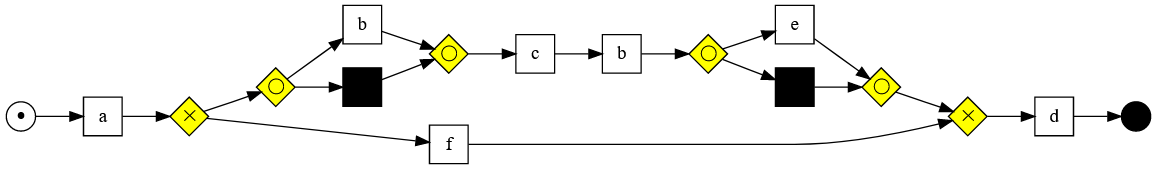
\includegraphics[scale=0.37]{model-example-correct.png}}
	\caption{\label{fig:flow_chart}Znaleziony model}
\end{figure}



Fitness:
0.9550392813257939
Metrics:
Alignment:	1.0
Complexity:	1
Generalization:	0.3426380039733623
Precision:	0.9874986894691236
Simplicity:	0.9230769230769231

Wykres działania w kolejnych generacjach:

\label{alignment-calculation}
Inne przykłady działania to: 

\section{Wyniki w zależności od przyjętych wag poszczególnych metryk}

\subsection{Złożoność}

\section{Wnioski}

\chapter{Podsumowanie}
Obie technologie przyszłościowe i wraz ze wzrostem mocy obliczeniowych.

Jest pole do rozwoju tak jak dla obu dziedziny 

Trzeba się trochę namęczyć

Wszystko się udało 

Złożoność można pewnie znaleźć lepszą, ale jest przepotężna i ma potencjał


% itd.
% \appendix
% \include{dodatekA}
% \include{dodatekB}
% itd.

\printbibliography

\end{document}
